%% 
%% Copyright 2007-2020 Elsevier Ltd
%% 
%% This file is part of the 'Elsarticle Bundle'.
%% ---------------------------------------------
%% 
%% It may be distributed under the conditions of the LaTeX Project Public
%% License, either version 1.2 of this license or (at your option) any
%% later version.  The latest version of this license is in
%%    http://www.latex-project.org/lppl.txt
%% and version 1.2 or later is part of all distributions of LaTeX
%% version 1999/12/01 or later.
%% 
%% The list of all files belonging to the 'Elsarticle Bundle' is
%% given in the file `manifest.txt'.
%% 
%% Template article for Elsevier's document class `elsarticle'
%% with harvard style bibliographic references

\documentclass[preprint,12pt,authoryear]{elsarticle}

%% Use the option review to obtain double line spacing
%% \documentclass[authoryear,preprint,review,12pt]{elsarticle}

%% Use the options 1p,twocolumn; 3p; 3p,twocolumn; 5p; or 5p,twocolumn
%% for a journal layout:
%% \documentclass[final,1p,times,authoryear]{elsarticle}
%% \documentclass[final,1p,times,twocolumn,authoryear]{elsarticle}
%% \documentclass[final,3p,times,authoryear]{elsarticle}
%% \documentclass[final,3p,times,twocolumn,authoryear]{elsarticle}
%% \documentclass[final,5p,times,authoryear]{elsarticle}
%% \documentclass[final,5p,times,twocolumn,authoryear]{elsarticle}

%% For including figures, graphicx.sty has been loaded in
%% elsarticle.cls. If you prefer to use the old commands
%% please give \usepackage{epsfig}

%% The amssymb package provides various useful mathematical symbols
\usepackage{amssymb}
%% The amsthm package provides extended theorem environments
%% \usepackage{amsthm}
\usepackage{float}
\usepackage{amsmath}
\usepackage[utf8]{inputenc}
\usepackage{url} 
\usepackage{hyperref}
\usepackage{xurl}
%% The lineno packages adds line numbers. Start line numbering with
%% \begin{linenumbers}, end it with \end{linenumbers}. Or switch it on
%% for the whole article with \linenumbers.
\usepackage{lineno}

%% creates acronyms but doesn't present them as a list at the start of the document.
\usepackage[nolist]{acronym}

%% allows for merging of vertical cells in tables
\usepackage{multirow}
\usepackage{array}

\journal{Canadian Journal of Forest Research}

\begin{document}

\begin{frontmatter}

%% Title, authors and addresses

%% use the tnoteref command within \title for footnotes;
%% use the tnotetext command for theassociated footnote;
%% use the fnref command within \author or \affiliation for footnotes;
%% use the fntext command for theassociated footnote;
%% use the corref command within \author for corresponding author footnotes;
%% use the cortext command for theassociated footnote;
%% use the ead command for the email address,
%% and the form \ead[url] for the home page:
%% \title{Title\tnoteref{label1}}
%% \tnotetext[label1]{}
%% \author{Name\corref{cor1}\fnref{label2}}
%% \ead{email address}
%% \ead[url]{home page}
%% \fntext[label2]{}
%% \cortext[cor1]{}
%% \affiliation{organization={},
%%            addressline={}, 
%%            city={},
%%            postcode={}, 
%%            state={},
%%            country={}}
%% \fntext[label3]{}

\title{The Role of Harvested Wood Products Half-life and Displacement Uncertainty in Forest Management Decision Trade-Offs and Carbon Dynamics in British Columbia}

%% use optional labels to link authors explicitly to addresses:
%% \author[label1,label2]{}
%% \affiliation[label1]{organization={},
%%             addressline={},
%%             city={},
%%             postcode={},
%%             state={},
%%             country={}}
%%
%% \affiliation[label2]{organization={},
%%             addressline={},
%%             city={},
%%             postcode={},
%%             state={},
%%             country={}}

\author[inst1]{Kathleen Coupland}

\affiliation[inst1]{organization={University of British Columbia, Faculty of Forestry and Environmental Stewardship},%Department and Organization
            addressline={2424 Main Mall}, 
            city={Vancouver},
            postcode={V6T 1Z4}, 
            state={British Columbia},
            country={Canada}}

\author[inst1]{Gregory Paradis}
\author[inst1]{Elaheh Ghasemi}
\author[inst1]{Salar Ghotb}
\author[inst1]{Walter Yan}

%%\affiliation[inst2]{organization={Department Two},%Department and Organization
%%            addressline={Address Two}, 
%%            city={City Two},
%%            postcode={22222}, 
%%            state={State Two},
%%            country={Country Two}}

\begin{abstract}
Forest carbon storage and sequestration is critically important when managing a forest for climate change resiliency. Through using a linear optimization forest model to project forest harvesting dynamics with the inclusion of both carbon stock tracking and the substitution effect on carbon emissions allows for a starting look at how these properties impact forest harvesting decisions. This project tested trade-off curves created by scenarios that maximized wood supply and those that maximized negative carbon emissions with a sequence of harvested wood product half-lives and displacement curves. These trade off curves were generated through model testing on a case study location in the central interior of British Columbia, Canada. 
Results showed that the model pushed towards either no harvesting (100\% retention) or quick rotation plantation style forestry (100\% clear-cutting), with no stable solution space for alternative silviculture systems. The highlights the importance of correct and accurate half-life and displacement value, but also indicates that having incorrect values may push harvesting activities in the opposite direction to minimize carbon emissions. Additionally, the results of this study indicate that silviculture systems that fall between 100\% harvest and 100\% retention may not be best suited for minimizing carbon emissions, which is contradictory to many prevailing assumptions about managing forests for carbon sequestration and storage. 
\end{abstract}

%%Graphical abstract
%%\begin{graphicalabstract}
%%\includegraphics{grabs}
%%\end{graphicalabstract}

%%Research highlights
\begin{highlights}
\item Research highlight 1
\item Research highlight 2
\end{highlights}

\begin{keyword}
%% keywords here, in the form: keyword \sep keyword
Forest management \sep Climate change mitigation \sep Carbon management \sep Harvested wood products \sep Displacement impact \sep linear optimization 
\end{keyword}

\end{frontmatter}

\begin{acronym}
   \acro{CO$_2$}{carbon dioxide}
   \acro{BC}{British Columbia}
   \acro{DOM}{dead organic matter}
   \acro{HWP}{harvested wood product}
   \acro{IPCC}{Intergovernmental Panel on Climate Change}
   \acro{GHG}{greenhouse gas}
   \acro{SFMM}{sustainable forest management model}
   \acro{FCBM}{forest carbon budget model}
   \acro{WPCM}{wood product carbon model}
   \acro{CBM-CFS3}{carbon budget model of the Canadian forest sector}
   \acro{UNFCCC}{United Nations Framework Convention on Climate Change}
   \acro{ws3}{Wood Supply Simulation System}
   \acro{SFM}{sustainable forest management}
   \acro{AOI}{area of interest}
   \acro{PG}{Prince George}
   \acro{TSA}{timber supply area}
   \acro{THLB}{timber harvesting land base}
   \acro{NTHLB}{non-timber harvesting land base}
   \acro{BEC}{biogeoclimatic zone}
   \acro{AU}{analysis unit}
   \acro{VDYP}{Variable Density Yield Projection}
   \acro{TIPSY}{Table Interpolation Program for Stand Yield}
   \acro{SBS}{Sub-Boreal Spruce}
   \acro{ESSF}{Englemann Spruce-Subapline Fir}
   \acro{SBS}{Sub-Boreal Spruce}
   \acro{BAFA}{ Boreal Alpine}
   \acro{ICH}{Interior Cedar-Hemlock}
   \acro{SWB}{ Spruce-Willow-Birch}
   \acro{SBPS}{Sub-Boreal Pine-Spruce}
   \acro{BWBS}{Boreal Black and White Spruce}
   \acro{MS}{Mountain Hemlock}
   \acro{IMA}{Interior Mountain-Alpine}
   \acro{LCA}{life-cycle assessment}

\end{acronym}

\begin{linenumbers}

%% main text
\section{Introduction}
\label{sec:introduction}
The interactions between  forest management paradigms and carbon dynamics are of increasing importance as the impacts of climate change are being realized (CITATION). Forests ability to remove atmosphere carbon and store carbon in biomass have been recognized as a having large climate change mitigation potential \citep{hurteau2021role}. Since 1990, it has been estimated that global forests have removed approximately one-third of the atmospheric \ac{CO$_2$} produced per year from the combustion of fossil fuels  \citep{pan2011large}. As trees accumulate biomass through photosynthesis, the carbon sequestered is distributed across multiple carbon pools, including above-ground biomass (leaves, branches, stems), below-ground biomass (roots, rhizomes), \ac{DOM}  (deadwood and litter), and soils. Using carbon pools, allows for the examination of differences in the amount of carbon stored in each pool and the rate in which carbon moves between different pools. Quantification of carbon storage, flux and flow in forested ecosystems is the starting point for determining how different forest management and \acp{HWP} change forest carbon dynamics. 

\subsection{forest management and how this impacts forest carbon and HWP}


\acp{HWP} are also an important component in how forests affect the carbon cycle, impacting the flux between stored carbon and the atmosphere. The rate at which carbon stored in \acp{HWP} is returned to the atmosphere depends on their type, usage, and end-of-life management \citep{skog1998carbon}. In 2013, the \ac{IPCC} updated guidelines to mandate the inclusion of the \acp{HWP} carbon pool when estimating total anthropogenic \ac{GHG} emissions and removals in the land-use, land-use change, and forestry sector \citep{hiraishi20142013}. Beyond carbon storage, \acp{HWP} can be a substitute for \ac{GHG}-intensive, non-renewable materials, such as concrete and steel, which are the most widely used construction materials globally \citep{geng2017review}, thereby reducing emissions through material substitution. In addition, wood-based bioenergy can replace fossil fuels and natural gas, providing an energy substitution effect \citep{geng2017review}. These substitutions highlight the potential of \acp{HWP} and the forest sectors role in mitigating climate change.

Quantifying forest resources and forecasting forest dynamics are fundamental to effective forest management planning [FIND CITATION]. Forest modeling has been extensively employed to help managers understand forest behavior, anticipate future changes, and make strategic, tactical, and operational decisions across spatial and temporal scales. Developing long-term strategies is essential for optimizing the use of finite forest resources while maintaining their ecosystem services \citep{martin2013optimization}. \Acp{SFMM} provide a framework for planning activities that address diverse objectives. Historically, \acp{SFMM}have focused on ensuring a continuous wood supply prioritizing  economic objectives. However, contemporary management emphasizes a balance between multiple objectives where wood supply, economics and ecosystem values (including carbon storage and sequestration), are managed concurrently \citep{gunn2007models}. 

To assess the impacts of forest management on carbon dynamics, balance timber and carbon objective trade-offs and identify optimal forest and timber management strategies, a robust forest carbon modeling framework is essential. Such a framework should integrate carbon indicators (e.g., total forest carbon stock and net forest carbon emissions) into \acp{SFMM} by linking them directly to existing \acp{FCBM} and \acp{WPCM}wood product carbon  model (WPCMs). While it is possible to conduct similar analyses manually by exporting the data generated from a \ac{SFMM} and using it as an input for a \ac{FCBM} and \ac{WPCM} for each time interval of interest, this approach is time-consuming, labor-intensive and only evaluates carbon and as a product of different forest management rather than as a manageable objective. 
In contrast, an integrated modeling framework enables efficient identification of management plans that satisfy multiple objectives and constraints via optimization algorithms. Historically, many \acp{SFMM} prioritized wood supply as the objective function, but over the past two decades, efforts have increasingly focused on maximizing forest carbon stocks to enhance climate mitigation.

\cite{meng2003combining} first incorporated carbon indicators into\acp{SFMM} by applying conversion factors from \ac{FCBM} to estimate biogenic carbon in commercial wood and soil. \cite{bourque2007optimizing} refined this approach by setting forest ecosystem carbon storage as an objective; however, they only considered two general carbon pools (biomass and soil) and used simplified conversion factors, limiting accuracy. Building on this, \cite{hennigar2008novel} and \cite{neilson2008optimal} integrated \ac{CBM-CFS3}, derived carbon yield curves representing detailed carbon pools, including softwood and hardwood biomass, DOM and snags, in \acp{SFMM}, enabling temporal modeling of ecosystem carbon stocks for different  types of stand. Their frameworks optimized ecosystem carbon stocks but did not consider \acp{HWP} or their substitution effects.

To date, no studies have explicitly optimized the total carbon stock of the forest system, including both ecosystem and \acp{HWP} pools, or aimed to minimize net carbon emissions across the entire forest sector. These gaps highlight opportunities to advance forest carbon management modeling. In addition, the carbon yield curve approach offers the potential to develop optimal strategies that simultaneously maximize total carbon stocks or minimize net emissions while meeting wood supply targets. 

This study aims to apply the carbon yield curve method previously proposed by \cite{hennigar2008novel, neilson2008optimal}. By developing a robust forest carbon management modeling framework, this research seeks to provide guidelines to optimize the potential to mitigate climate change in forest sectors. Carbon indicators for total forest carbon stock and net forest carbon emissions have been calculated and built into the \ac{SFMM} with the carbon yield curve method. 

The reminder of this paper is organized as follows. Section \ref{sec:methods} presents the methodological approach adopted in this study. Section \ref{sec:case-study} describes the case study and data. Section \ref{sec:results} reports the results, followed by a discussion in Section \ref{sec:discussion}, Finally, Section \ref{sec:conclusion} provides concluding remarks. 




Forest management can play a pivotal role in climate change mitigation and sustainable development options, through intentional interventions that impact the forest carbon cycle. In 2007, the \ac{IPCC} recognized all scales of forest management (plot to landscape) as a critical nature-based climate change mitigation strategy.  \citep{Nabuurs2007Forestry}. 
in the forest ecosystem and through ensuring production of \acp{HWP} with longer product life-cycles.
Climate change, defined as persistent alterations in temperature and weather patterns, has been driven predominantly by rising \ac{GHG} emissions from anthropogenic activities since the Industrial Revolution \citep{UNClimateChange2024}. In response to the growing challenge of climate change,  the United Nations established the \ac{IPCC} in 1988 \citep{IPCCwebsite}, which subsequently led to the creation of the \ac{UNFCCC} in 1992 \citep{UNFCCCWebpage}. The Kyoto Protocol, adopted in 1997, operationalized the \ac{UNFCCC} by introducing legally binding emission reduction targets for participating countries \citep{UNFCCC_History}. A pivotal advancement was the adoption of the Paris Agreement in 2015, which aimed to limit global temperature rise to below $2^{\circ}\text{C}$ above preindustrial levels \citep{UNFCCC_Paris_Agreement}. The agreement required all parties to implement mitigation measures, reduce \ac{GHG} emissions, and ultimately work towards achieving net-zero emissions.

 The \ac{IPCC} further emphasized: “In the long term, a sustainable forest management strategy aimed at maintaining or increasing forest carbon stocks, while producing an annual yield of wood, fiber, or energy from the forest, will generate the largest sustained mitigation benefit” \citep{Nabuurs2007Forestry}. Accordingly, forest carbon management encompasses the actions, plans, and strategies implemented to systematically maintain or increase carbon stocks or sequestration across the entire forest sector, accounting for both forest ecosystems and \acp{HWP}.

\section{Methods}
\label{sec:methods}
\subsection{Overview}
\label{sec: overview} 
This study aims to develop a forest carbon management modeling framework to identify forest management strategies that optimize the climate change mitigation potential of forest sectors. To assess the climate impacts of various forest management strategies, the framework integrates the \ac{ws3} to simulate forest growth and optimize forest management activities \citep{Paradis_ws3_a_Wood_2025}, and libCBM \citep{libcbmpy} to estimate long-term carbon stocks and flows within forest ecosystems. \ac{ws3} is an open-source forest estate modeling tool implemented in Python, developed to support \ac{SFM} planning and forest resource analysis. For carbon accounting, the study utilizes libCBM, an open-source implementation of the \ac{CBM-CFS3} \citep{KURZ2009480}, to estimate carbon stocks and their temporal changes within forest ecosystems. To simulate the carbon dynamics of \acp{HWP}, this study integrates the modeling of product pool decomposition with the assessment of substitution effects associated with \acp{HWP}. This study presents and integrative modeling framework to optimize forest management decisions under maximizing carbon stocks and minimizing net carbon emissions.  

Figure \ref{framework} provides an overview of the modeling process used in this study, which is divided into three main stages: data preparation, model execution, and modeling output comparison. The data preparation stage includes an \ac{AOI}, forest inventory data preparation, development of both timber yield and carbon yield curves and compiling \ac{HWP} data. The second stage includes the building of the modeling framework and integration of \ac{ws3} and the \ac{WPCM} to simulate various forest management scenarios. The model objective is twofold: (1) to maximize total carbon storage across both forest ecosystems and harvested wood products, and (2) to minimize net carbon emissions from the entire forest system, accounting for the climate mitigation benefits associated with product substitution. Finally, in the third stage, the optimized outputs generated by the modeling framework are compared against baseline results obtained from libCBM, in order to evaluate the consistency and effectiveness of the proposed approach for modeling carbon within a linear optimization forest supply timber analysis framework.

\begin{figure}[t]
    \centering
    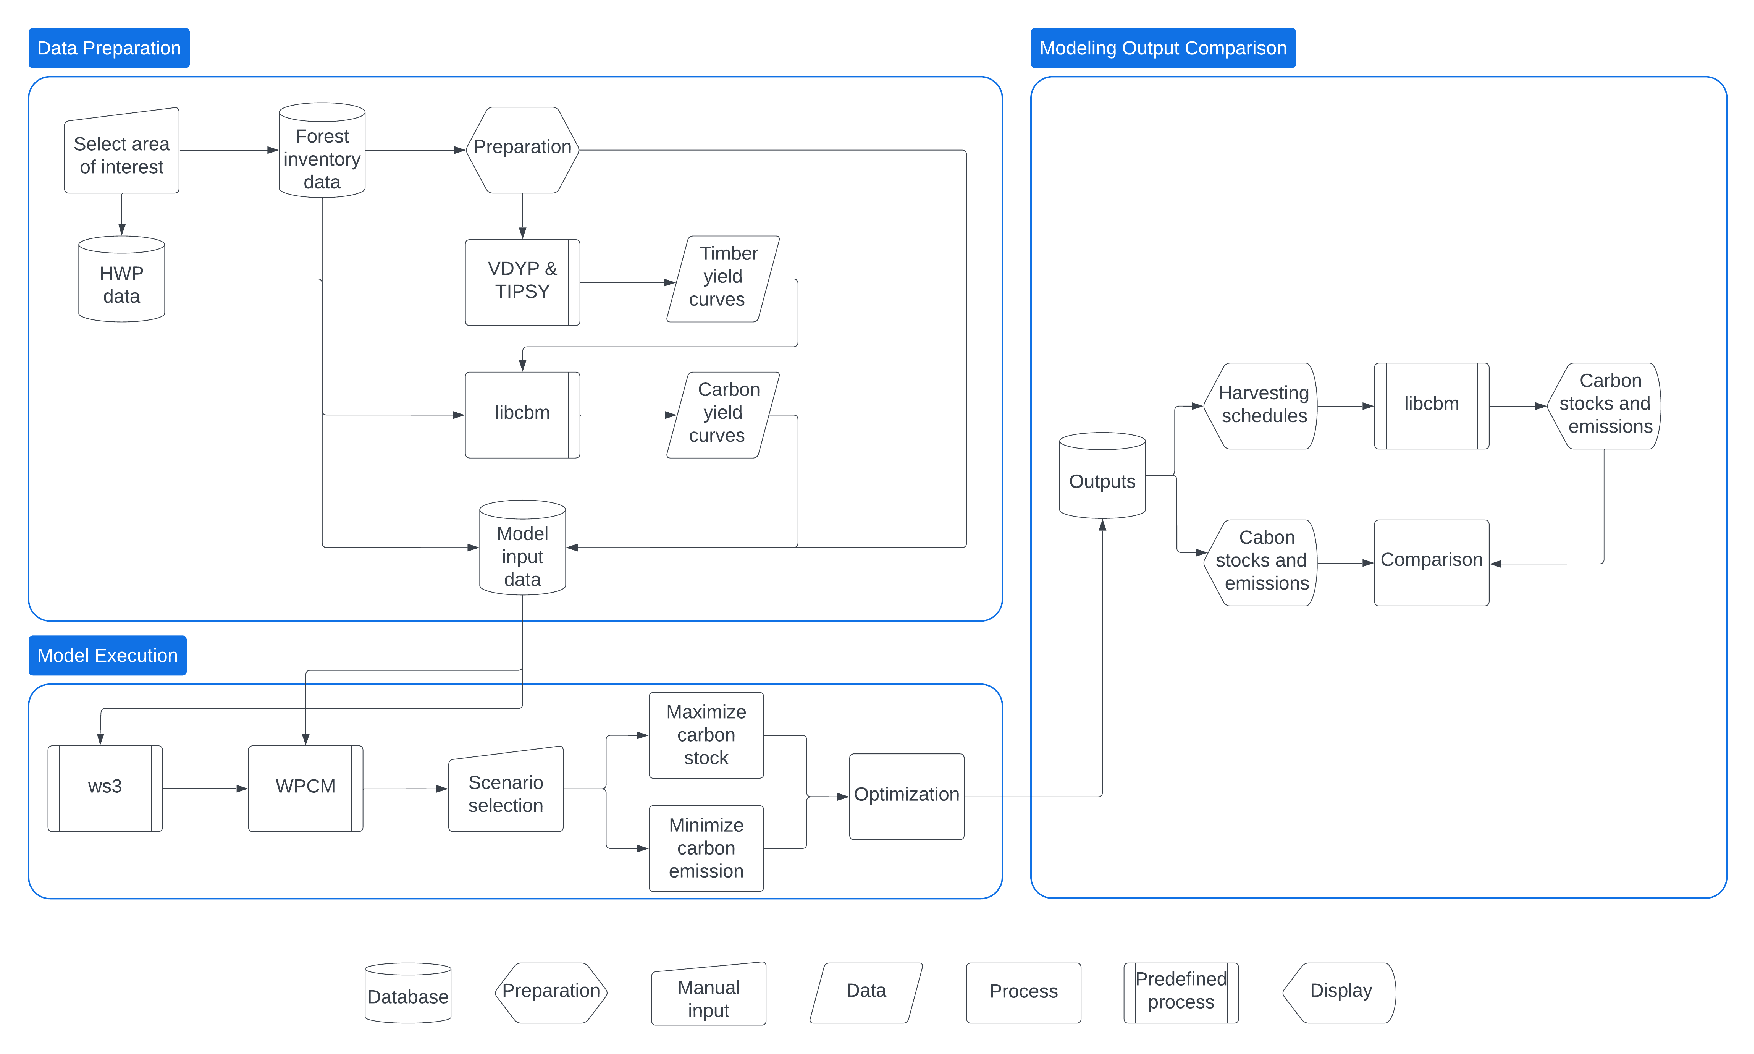
\includegraphics[width=1\linewidth]{framework.pdf}
    \caption[The integrated forest carbon management modeling framework.]{The integrated forest carbon management modeling framework}
    \label{framework}
\end{figure}

\subsection{Modeling framework}
\label{sec:modeling-framework}
\subsection{Data Preparation}
\label{sec:case-study}
\subsubsection{Area of Interest}
 The \ac{PG} \ac{TSA}, located in the north-central interior of \ac{BC}, Canada, was selected as the case study site (Figure \ref{fig: TSA24_AOI}). The \ac{PG}-\ac{TSA} covers 7.97 million ha, is one of the largest management units in \ac{BC} and has forest types representative of \acp{BC} interior. It contains $\approx$ 15\% of the provincial \ac{THLB} highlighting its economic importance to the \ac{BC} timber industry \citep{princegeorge2017}. 
 
\begin{figure}[H]
    \centering
    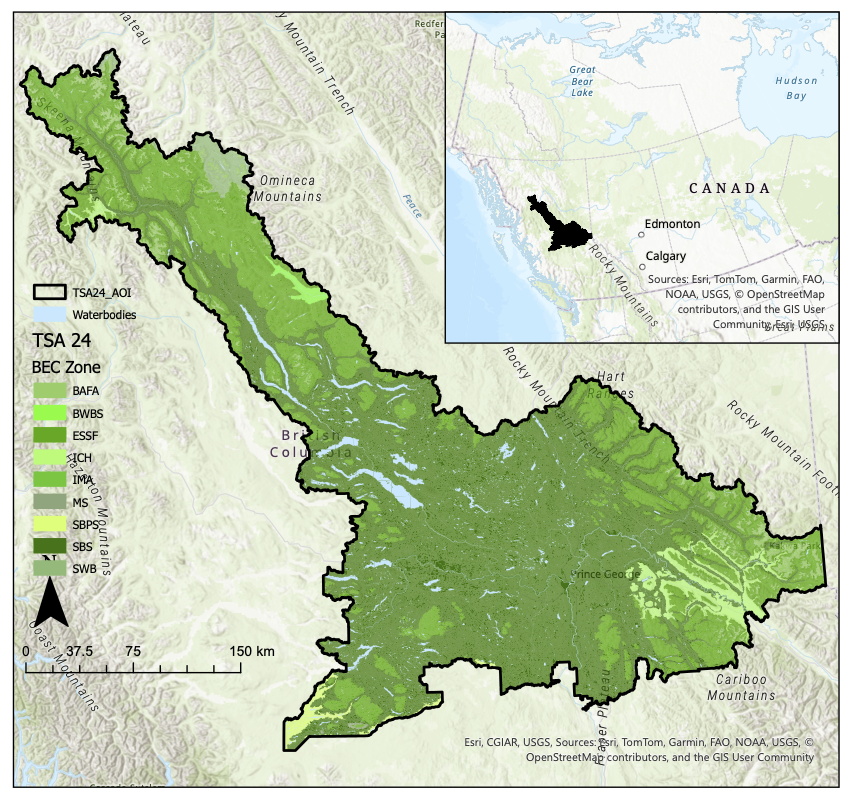
\includegraphics[width=1\linewidth]{TSA24_AOI.png}
    \caption{Study area indicating the Prince George TSA.}
    \label{fig: TSA24_AOI}
\end{figure}
\subsubsection{Forest Inventory Data}
After selecting the \ac{PG}-\ac{TSA} as the \ac{AOI} for this study, the relevant forest inventory data was procured. This forest inventory data was collected, processed and prepared in a previous study by \citep{boisvenue2022managing}.  The forest inventory includes stand-level attributes, such as stand area, age, leading species composition, site index, \ac{BEC} and delineation in to the \ac{THLB} and \ac{NTHLB}. Leading species, site index and \ac{BEC} were used to stratify the land base in to \acp{AU}. The \ac{AU} classification were the base unit used to determine both timber and carbon yield curves. Every \ac{AU} in the \ac{PG}-\ac{TSA} was assigned a timber type, this ensures that every \ac{AU} has both a timber and carbon curve. The forest inventory preparation also included descriptive statistics about the characteristics of the \ac{AOI}. 

\subsubsection{Yield Curves}
Two sets of yield curves were needed for this study: timber yield curves and carbon yield curves. The timber yield curves had been previously created in from \citep{boisvenue2022managing} study. The yield curves used were divided into two groups. \Ac{VDYP} model generated the timber yield curves for previously unmanaged stands and \ac{TIPSY} program for the generation of timber yield curves managed stands. Managed vs unmanaged stands were separated based on previous regeneration practices. If the stand had been previously harvested and planted it was considered managed and if the stand was not planted and natural regeneration was allowed to occur the stand was considered unmanged. Timber yield curves were projected for a 350-year planning horizon. All \acp{AU} were assigned a starting yield curve and a transition curve that gets applied after harvest occurred. 

Carbon yield curves were created following \citep{neilson2008optimal}, integrating carbon into the \ac{SFMM} alongside the timber yield curves. Forest carbon was modelled with libCBM, the open-source implementation of \ac{CBM-CFS3} \citep{KURZ2009480}, across 21 carbon pools (10 biomass and 11 \ac{DOM}) and 52 carbon fluxes. For each analysis unit, a one-hectare stand was simulated on its natural trajectory to the model's typical harvest age (120 years; the area-weighted median harvest age measured under the even-flow scenarios), at which point a clearcut harvest event transferred the carbon pools according to CBM's disturbance matrix (merchantable carbon removed; slash and dead roots transferred to the \ac{DOM} pools), and the stand regrew on its managed yield curve. Repeating the harvest at the rotation age until the \ac{DOM} pools reached their cycle equilibrium, and extracting the post-harvest trajectory, yielded the managed carbon yield curves; the natural curves are the no-management trajectories. The projections were aggregated into biomass, merchantable, \ac{DOM} and ecosystem stock curves and one net emission flux curve. This structure allows for carbon to be integrated in the \ac{SFMM} similar to the integration of timber yield curves. Aggregating the carbon curves and fluxes allowed for computational efficiency and sufficient carbon yield accuracy for simulation and optimization. Additionally, this method leaves space for more detailed or additional carbon pools and fluxes to be added in later studies. 

Dead organic matter initialization in \ac{CBM} is known to produce upward-biased initial pools: the initialization procedure applies stand-replacing disturbances at regular intervals equal to the fire return interval rather than the stochastic disturbance regime, which over-accumulates carbon relative to the landscape's carbon-holding capacity \citep{boisvenue2022managing}, and initialization choices are a documented source of variation and systematic error in carbon models \citep{metsaranta2017, oberpriller2021}. Because a post-harvest reset to the initialized state would inherit this bias, the managed curves in this study are generated by simulating the harvest itself, so that post-harvest carbon states are conservation-consistent with the harvested stand's pre-harvest state; the residual difference between first-rotation and steady-state harvest histories is about 1\% of landscape carbon. 

\subsubsection{HWP Data}
This study assumed an 85\% utilization amount of harvested wood \citep{smyth2020climate}. The utilized fiber was divided into two equal categories of \acp{HWP}: paper and solid wood products \citep{ipcc2019refinement}. This division of \acp{HWP} was determined based off of historical data on log availability and utilization in \ac{BC} \cite{BC_Mill_List_2020}  An average wood density ($0.46 \, \text{ton/m}^3$) was adopted from \citep{kennedy1965strength}, along with a conversion factor of 0.5 tC per 1 t of dry wood to estimate carbon content \citep{penman2003good}. 
\Ac{LCA} data  required to parameterize the \ac{WPCM}, including \ac{HWP} half-lives and displacement factors, were obtained from \citep{smyth2020climate}. The half-life of paper products was assumed to be 2 years, while that of solid wood products was assumed to be 30 years \citep{eggleston2006ipcc}. These values were used to derive the annual decay constants for first-order decay \citep{eggleston2006ipcc}. According to previous literature, the default displacement factor is 2.2 tC/tC for solid wood products and 0 tC/tC for paper products \cite{smyth2020climate}. 

\subsubsection{The Sustainable Forest Management Model}
\label{sec: modeling}
This study employed \ac{ws3} which integrates the forest inventory data, timber and carbon yield curves, management actions, transitions and scenario parameters to construct a \ac{SFMM} for simulation and optimization. The optimization model applied in this study to achieve the objective functions and satisfy the constraints across different scenarios was adapted from the work presented of \citep{paradis2013risk}. 

The mathematical formulation of the proposed model is presented as follows:
\begin{align}
\text{max} & \quad \sum_{i \in Z} \sum_{j \in J_i} c_{ij} x_{ij} \label{eq:1} \\
\text{s.t.} & \quad \sum_{j \in J_i} x_{ij} = 1, \quad \forall i \in Z \label{eq:2} \\
& \quad (1 - \epsilon_p) y_{p1} \leq \sum_{i \in Z} \sum_{j \in J_i} \mu_{ijpt} x_{ij} \leq (1 + \epsilon_p) y_{p1}, \quad \forall p \in O', t \in T \label{eq:3} \\
& \quad v_{ot}^- \leq \sum_{i \in Z} \sum_{j \in J_i} \mu_{ijot} x_{ij} \leq v_{ot}^+, \quad \forall o \in O, t \in T \label{eq:4} \\
& \quad 0 \leq x_{ij} \leq 1, \quad \forall i \in Z, j \in J_i \label{eq:5}
\end{align}
where:
\begin{align*}
Z &:= \text{set of spatial zones} \\
J_i &:= \text{set of available prescriptions for zone } i \in Z \\
O &:= \text{set of forest outputs} \\
O' &\subseteq O := \text{set of targeted forest outputs} \\
T &:= \text{set of periods in the planning horizon} \\
\epsilon_p &:= \text{admissible level of variation on yield of targeted output } p \in O' \\
\mu_{ijot} &:= \text{quantity of output } o \in O \text{ produced in period } t \in T \notag \\
           &\quad \text{by prescription } j \in J_i \text{ in zone } i \in Z \\
v_{ot}^- &:= \text{lower bound on yield of output } o \in O \text{ in period } t \in T \\
v_{ot}^+ &:= \text{upper bound on yield of output } o \in O \text{ in period } t \in T \\
c_{ij} &:= \text{objective function contribution of prescription } j \in J_i \text{ in zone } i \in Z \\
x_{ij} &:= \text{proportion of zone } i \in Z \text{ on which prescription } j \in J_i \text{ is applied} \\
y_{p1} &:= \sum_{i \in Z} \sum_{j \in J_i} \mu_{ijp1} x_{ij}, \notag \\
       &\quad \text{i.e. first-period harvest volume for targeted output } p \in O'
\end{align*}
The objective function (\ref{eq:1}) maximizes the desired result based on the applied prescriptions. For this study a no harvest option (i.e. do nothing) was considered a valid prescription  in addition to more standard prescriptions, including harvesting.  Constraint sets specify that the total proportion of prescriptions applied to each zone must be equal to one  (\ref{eq:2}) . Then an even-flow constraint set was created that ensured consistency in target outputs (\ref{eq:3}).  Constraint sets  enforce upper and lower bounds on the yields in each period (\ref{eq:4}). The domain of the decision variables is defined by constraint sets (\ref{eq:5}).

{The Wood Product Carbon Model}
\label{sec: wood model}
The \ac{WPCM} developed for this study serves two primary functions: (1) tracking the carbon stocks and the emissions associated with \acp{HWP} derived from harvested timber over the simulation horizon, and (2) estimating the substitution effects of  \acp{HWP}. The constraints are same as those defined in the \ac{SFMM}. Additionally, the constraints sets are identical to those defined in the \ac{SFMM}; however, the objective function is reformulated to either maximize carbon stocks or minimize net emissions.

\paragraph{Maximize the Total Forest System Carbon Stock}
This objective is to maximize the total carbon stock of the entire forest system (Eq. \ref{eq:6}), where the total carbon stock is defined as the sum of the carbon stored in the forest ecosystem and in \acp{HWP} (Eq. \ref{eq:7}). 

\begin{align}
\max \sum_{t \in T} C_t^{\text{sys}}
\label{eq:6}
\end{align}

\begin{equation}
C_t^{\text{sys}}= C_t^{\text{eco}}+ C_t^{\text{hwp}}
\label{eq:7}
\end{equation}

where,
\begin{align*}
C^{\text{sys}}_t &:= \text{Carbon stock of the entire forest system in period } t \in T\\
C^{\text{eco}}_t &:= \text{Carbon stock of the forest ecosystem in period } t \in T\\
C^{\text{hwp}}_t &:= \text{Carbon stock of all {HWP} in period } t \in T
\end{align*}

Carbon stock of all \acp{HWP}, $C^{\text{hwp}}_t$, is defined through Eq.~\ref{eq:8} to Eq.~\ref{eq:11}.


\begin{equation}
C^{\text{hwp}}_t = \sum_{p \in P}C_{\text{p,t}}
\label{eq:8}
\end{equation}

\begin{equation}
C_{\text{p,t}} = a_{\text{p}}C_t^{\text{wood}}
\label{eq:9}
\end{equation}

\begin{equation}
C_t^{\text{wood}} = \rho^{\text{wood}} V_t C^{\text{content}}
\label{eq:10}
\end{equation}

\begin{equation}
\sum_{p \in P}a_{\text{p}} = 1
\label{eq:11}
\end{equation}

where,

\begin{align*}
    P &:= \text{Set of products} \\
    V_t &:= \text{Volume of harvested wood in period $t \in T$ (m}^3\text{)} \\
    \rho^{\text{wood}} &:= \text{Wood density (ton/m}^3\text{)} \\
    C^{\text{content}} &:= \text{Carbon content of the wood} \\
    C^{\text{wood}} &:= \text{Carbon stock of harvested wood (ton)} \\
    C_{\text{p,t}} &:= \text{Carbon stock of product $p \in P$ in time period $t \in T$ (ton)} \\
    a_{\text{p}} &:= \text{Allocation factor for product $p \in P$}
\end{align*}

Once a \ac{HWP} enters its life cycle, the \ac{IPCC} first-order decay model \citep{eggleston2006ipcc} is applied to calculate changes in the \ac{HWP} carbon stocks over time  (Eq. \ref{eq:12}). The half-life of each product is then used to determine the corresponding annual decay constants in the first-order decay model (Eq. \ref{eq:13}).

\begin{equation}
C_{\text{p,t+1}} = C_{\text{p, t}}(1 - k_{\text{p}})^{10}
\label{eq:12}
\end{equation}

\begin{equation}
k_{\text{p}} = \frac{\ln(2)}{hl_{\text{p}}}
\label{eq:13}
\end{equation}

where,
\begin{align*}
    k_{\text{p}} &:= \text{Annual decay constant of first-order decay for product $p \in P$} \\
    hl_{\text{p}} &:= \text{Half-life for product $p \in P$ in years} \end{align*}


\paragraph{Minimize the Net Forest Carbon Emission}
The objective function (Eq. \ref{eq:14}) minimizes the net carbon emissions from the forest sector, defined as the sum of carbon emissions from the forest ecosystem and \acp{HWP}, minus the substitution effect of \acp{HWP} (Eq. \ref{eq:15}). 
The accounting is implemented as a stock-difference formulation, $E_{sys}(t) = [E(t) - E(t+1)] + [H(t) - H(t+1)] - S_t^{\text{hwp}}$, where $E(t)$ and $H(t)$ are the ecosystem and harvested wood product carbon stocks at period $t$, so that summing over the planning horizon telescopes exactly to the total system carbon change minus the substitution effect; the objective is therefore carbon-conservative by construction. The harvested wood product ledger tracks product pools only (harvest residue and field losses are inside the ecosystem stock change), with the utilized fibre split equally between paper and solid wood products as described above. 

\begin{align}
\min \sum_{t \in T} E_t^{\text{sys}}
\label{eq:14}
\end{align}

\begin{equation}
E_t^{\text{sys}} = \frac{44}{12}(E_t^{\text{eco}}+ E_t^{\text{hwp}} - S_t^{\text{hwp}})
\label{eq:15}
\end{equation}



where,
\begin{itemize}
    \item $E_t^{\text{sys}}$ := $ \mathrm{CO}_2 $ emission of the whole forest system in the period $t \in T$.
    \item $E_t^{\text{eco}}$ := $ \mathrm{CO}_2 $ emission of the forest ecosystem in the period $t \in T$.
    \item $E_t^{\text{hwp}}$ := $ \mathrm{CO}_2 $ emission of all \acp{HWP} in the period $t \in T$.
    \item $S_t^{\text{hwp}}$ := Substitution effect of all \acp{HWP} in the period $t \in T$.
\end{itemize}

In this study, \acp{HWP}carbon emissions, $E_t^{\text{hwp}}$, are calculated from annual changes in carbon stocks within each \acp{HWP} pool. The emitted carbon is subsequently converted to \ac{CO$_2$} as shown in Eq. (\ref{eq:16}).
\begin{equation}
E_{t+1}^{\text{hwp}} = \frac{44}{12}(C_{t+1}^{\text{hwp}}- C_t^{\text{hwp}})
\label{eq:16}
\end{equation}
The substitution effect of\acp{HWP}, $S_t^{\text{hwp}}$, is calculated using their displacement factors (Eqs. \ref{eq:17} and \ref{eq:18}). 
\begin{equation}
S_t^{\text{hwp}} = \sum_{p \in P}S_{\text{p,t}}
\label{eq:17}
\end{equation}

\begin{equation}
S_{\text{p,t}} = C_{\text{p,t}}df_{\text{p}}
\label{eq:18}
\end{equation}
where, 
\begin{align*}
    S_{\text{p,t}} &:= \text{Substitution effect for product $p \in P$ in period $t \in T$} \\
    df_{\text{p}} &:= \text{Displacement factor for product $p \in P$ } \end{align*}

\subsection{Model Execution}
\label{sec: Model Execution}
For the simulations and optimizations in this study, a 200-year time horizon (beginning in 2020) was adopted and divided into 20 periods of 10 years each. In each optimization problem, the even-flow constraints were applied to both harvest volume and harvest area, restricting their variation between consecutive periods to less than 5\%.

\subsubsection{Carbon Stocks}
Unlike conventional carbon accounting approaches, this study approximates forest carbon stocks and emissions and integrates them with the optimization model. Thus, it is necessary to evaluate and compare the model outputs directly to the forest carbon budget model results. This was done through creating two landscape-level tests that applied no-harvest and max-harvest constraints, allowing for direct comparison of the carbon outputs from the new proposed model to the reference model libcmb.

\subsubsection{Half-life and Displacement Sensitivity Analysis}
To assess the impact of \acp{HWP} and displacement, we consider the outputs of a bi-objective optimization model and assessed the impacts of different half-lives and displacement factors on the carbon emission and harvest volume objectives.  the half-life ranges from 30 to 60 years and the displacement factor varies between 0 and 1.5. 
Since the intensity of trade-offs is influenced by the half-life and displacement factor, it is important to conduct sensitivity analysis on these parameters. Therefore, 5,000 scenarios were simulated by varying the half-life values from 1 to 200 and the displacement factor from 0 to 2.4 with 0.1 steps. 
\newpage
\section{Results}
\label{sec:results}
\subsection{Forest Inventory}
The \ac{THLB} is predominantly coniferous, with lodge-pole pine (\textit{Pinus contorta}) accounting for 49\%, spruce (\textit{Picea spp.}) for 33\%, subalpine fir (\textit{Abies lasiocarpa}) for 9\%, Douglas fir (\textit{Pseudotsuga menziesii}) for 2\%, and cedar (\textit{Cedrus spp.}) for 1\%. 
The \ac{PG}-\ac{TSA} is composed of two main \acp{BEC}: \ac{SBS} (62.2\%) and \ac{ESSF} (28.7\%). The remaining 9\% of the land base is composed of \ac{BAFA} (3.7\%), \ac{ICH} (2.8\%), \ac{SWB} (1.2\%), \ac{SBPS} (0.9\%), \ac{BWBS} (0.4\%), \ac{MS} (0.05\%), and \ac{IMA} (0.02\%). Approximately 44\% of the study area, about 3.10 milion hectares of crown forest land, is classified as the \ac{THLB}, defined as forest land acceptable and economically feasible for timber harvest \citep{bcfpb_glossary}. The remaining area consists of regions with low timber volume, low site productivity, and accessibility challenges (e.g., steep slopes, remote locations lacking road infrastructure) that make them economically unattractive or infeasible under current market conditions \citep{princegeorge2017}. Additional areas were excluded from the \ac{THLB} for legal, ecological or cultural reasons including parks, protected areas (e.g., wildlife habitat), riparian zones (lakes, rivers, wetlands, and streams), and sites of cultural significance (e.g., Indigenous archaeological sites) \citep{princegeorge2017}. 
Using the forest inventory data, the study area was stratified into 24 distinct \acs{AU}. Of the 24 \acs{AU}, 11 were for unmanaged forests (\ac{THLB} = 0) and 13 for managed forests (\ac{THLB} = 1). The species composition by area (ha) for unmanaged forests (outside the \ac{THLB}) and managed forests (within the \ac{THLB}) are summarized in Figure \ref{fig: unmanaged species structure} and Figure \ref{fig: managed species structure}. 
\begin{figure}[H]
    \centering
    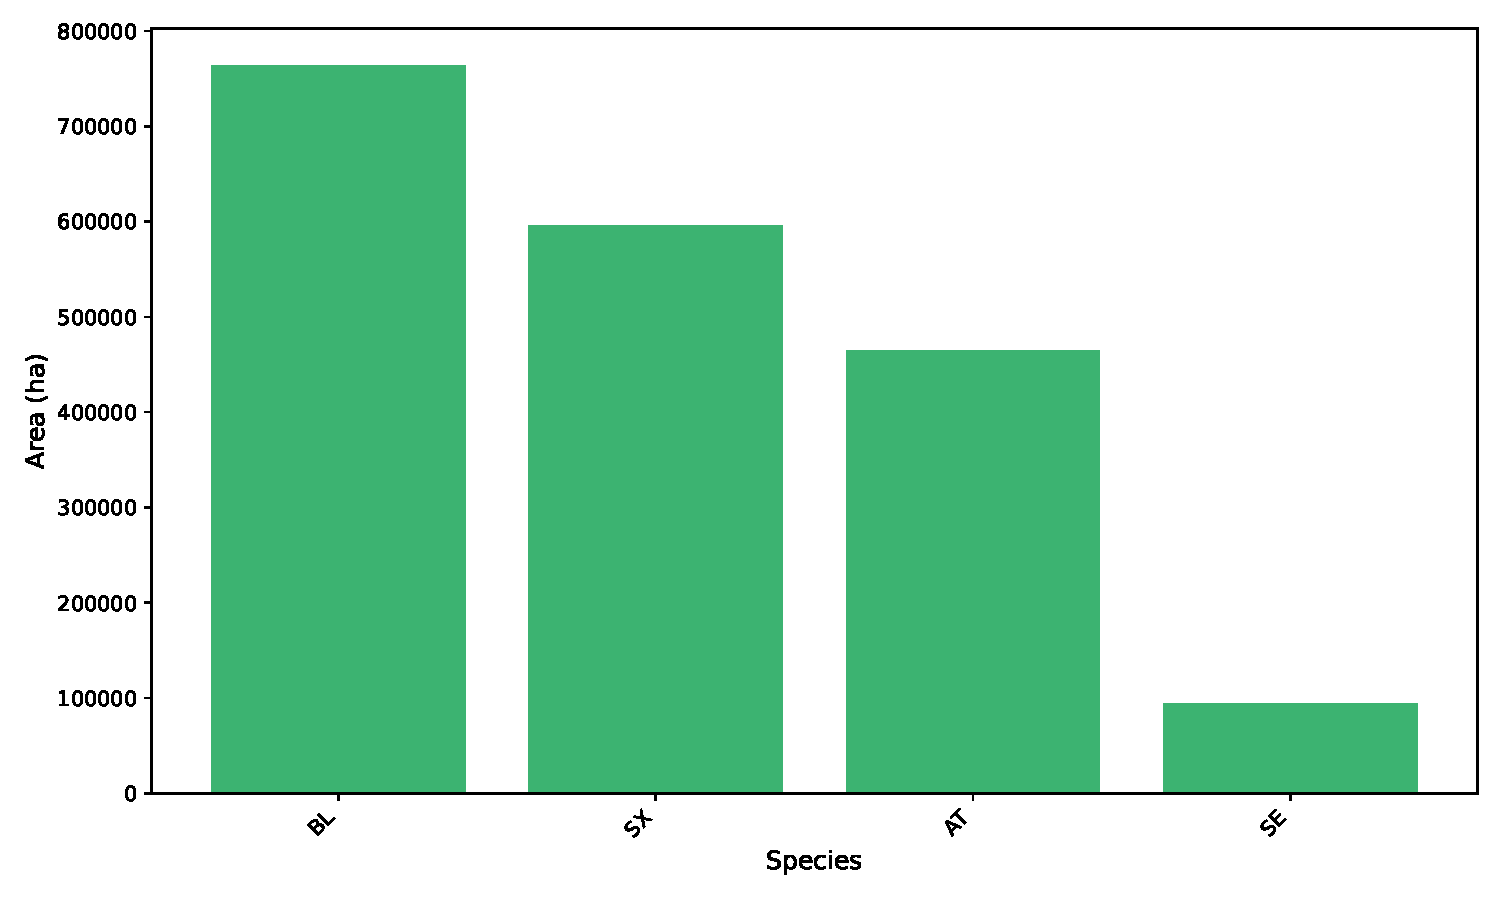
\includegraphics[width=0.9\linewidth]{leading_species_structure_unmanaged.pdf}
    \caption[Species composition of unmanaged forests in TSA 24.]{Species composition of unmanaged forests in TSA 24. \\ AT = Trembling Aspen (\textit{Populus tremuloides}), BL = Subalpine Fir (\textit{Abies lasiocarpa}), SE = Engelmann Spruce (\textit{Picea engelmannii}), and SX = Spruce Hybrid (\textit{Picea engelmannii × Picea glauca}).}
    \label{fig: unmanaged species structure}
\end{figure}
\begin{figure}[H]
    \centering
    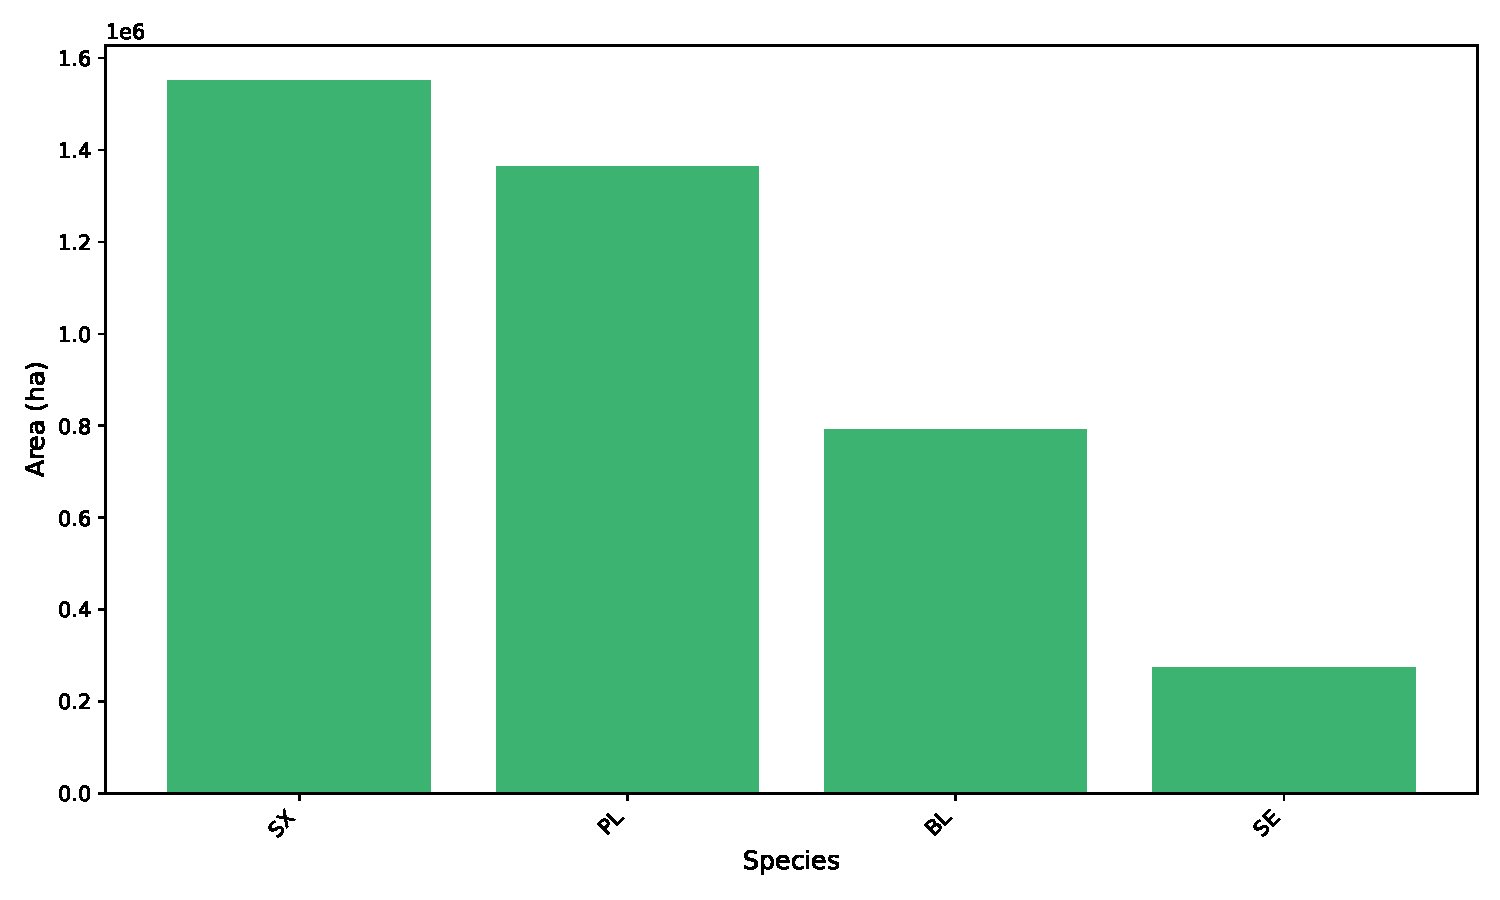
\includegraphics[width=0.9\linewidth]{leading_species_structure_managed.pdf}
    \caption[Species composition of managed forests in TSA 24.]{Species composition of managed forests in TSA 24. \\ PL = Lodgepole Pine (\textit{Pinus contorta}), SX = Spruce Hybrid (\textit{Picea engelmannii} $\times$ \textit{Picea glauca}), BL = Subalpine Fir (\textit{Abies lasiocarpa}), and SE = Engelmann Spruce (\textit{Picea engelmannii})}
    \label{fig: managed species structure}
\end{figure}
In unmanaged forests, Subalpine Fir occupies the largest area, followed by Hybrid Spruce, Trembling Aspen, and Engelmann Spruce. In managed forests, the composition shifts, with Hybrid Spruce being the most extensive, followed by Lodgepole Pine, Subalpine Fir, and Engelmann Spruce.

The age structure and area distribution of unmanaged and managed forests in \ac{TSA} 24 are summarized in Figure~\ref{fig: unmanaged age structure} and Figure \ref{fig: managed age structure}, respectively. Unmanaged forests exhibit a board age range, from very young stands to those approaching 500 years, with a relatively even area distribution across age classes. In contrast, managed forests display a narrower age range, predominantly up to 400 years, with distinct peaks at specific age intervals. 

\begin{figure}[H]
    \centering
    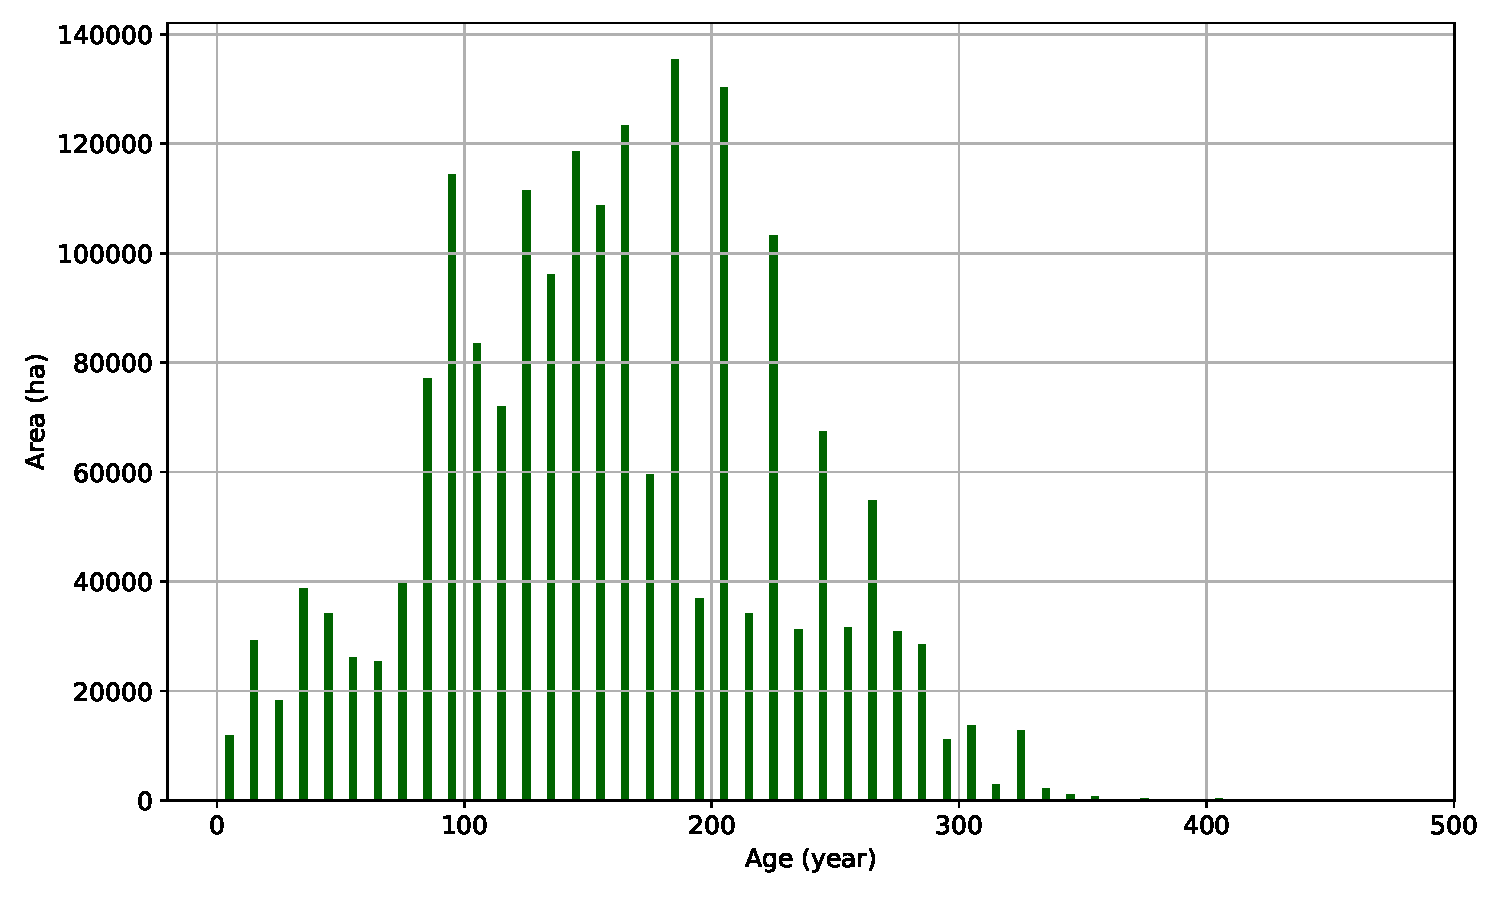
\includegraphics[width=1\linewidth]
    {area_distribution_unmanaged.pdf}
    \caption[Age structure distribution of unmanaged forests in TSA 24.]{Age structure distribution of unmanaged forests in TSA 24.}
    \label{fig: unmanaged age structure}
\end{figure}

\begin{figure}[H]
    \centering
    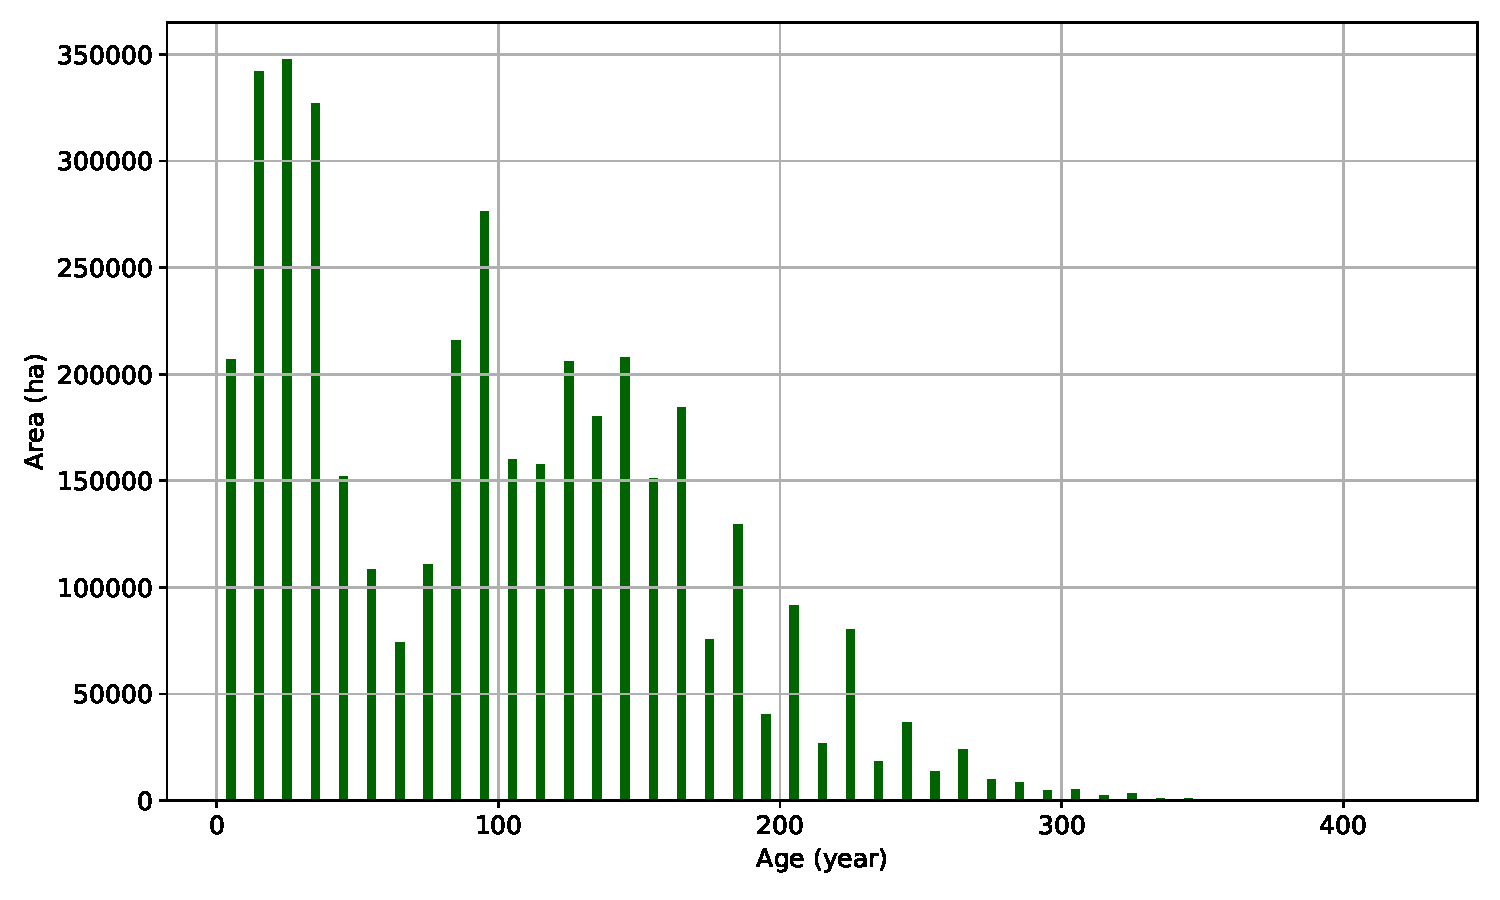
\includegraphics[width=1\linewidth]
    {area_distribution_managed.pdf}
    \caption[Age structure distribution of managed forests in TSA 24.]{Age structure distribution of managed forests in TSA 24.}
    \label{fig: managed age structure}
    \end{figure}
\subsection{Model Performance}
\label{sec: Model performance}
The \ac{SFMM} developed allows for users to set various objectives. 
\subsection{Maximize Harvest Volume}
When harvesting volume is maximized, harvest area ranges from 369000 to 408000 $ha/period$ and harvest volume ranges from  $7.45\times10^7$ $m^3/period$ and $8.23\times10^7$ $m^3/period$. Growing stock ($m^3$) decreases  from x to x. 


\begin{figure}
    \centering
    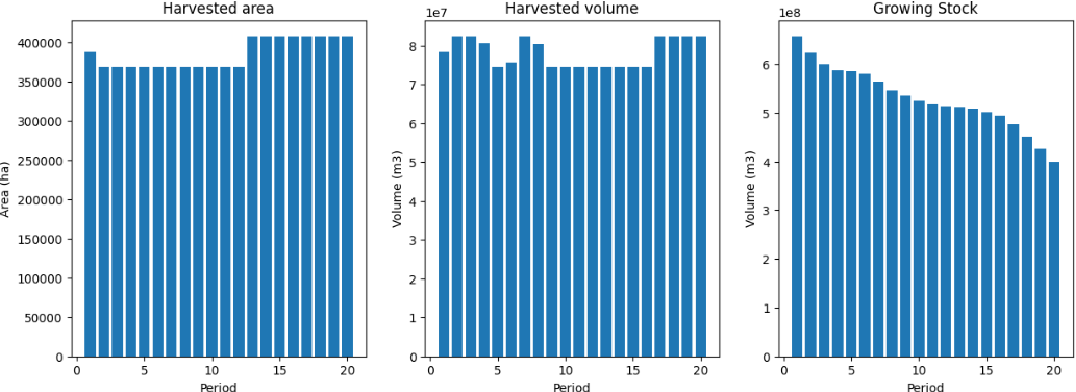
\includegraphics[width=1\linewidth]{hs_mh.pdf}
    \caption{The amount of harvested volume, harvested area, and growing stock over the 200-year planning horizon under maximize harvest volume scenario.}
    \label{fig: area_vol_stock}
\end{figure}

\subsection{Maximize Total Forest System Carbon Stock}
\subsection{Minimize Net Forest Carbon Emissions}
Results for these two sections haven't been reported. Will follow the same reporting structure as before. 

\subsection{Carbon Stocks}
\subsubsection{No Harvest}
In the no-harvest scenario, the initial total carbon stored three carbon stocks from \ac{ws3} and libcbm are presented in table \ref{tab:No harvest emissions} . These values are also represented graphically in \ref{fig: nh_stock} , showing the deviations between the two models through time. The \ac{DOM} carbon stock shows a slow increase across the planning horizon and only a slight variation between the two models from period 2 through 11. However, all differences were under 2\% and deemed negligible and with standard model variability.. The biomass carbon stock exhibited a faster growth in the first 8 periods followed by a slight decline through to the end of the planning horizon. The initial values of the biomass carbon stock were slightly different between \ac{ws3} and libcbm with ws3 being $+$ $0.029 \times 10^{9}$ (7.1\%). This difference is less than 1\% at period 10.  Of note is that the variations between the models is minor and the overall pattern of carbon accumulation in the ecosystems is the same. 
\begin{table}[h!]
    \centering
    \begin{tabular}{cccc>{\centering\arraybackslash}p{0.2\linewidth}}
         Carbon Stock $tC$&&   ws3&libcbm &Average difference (\%)\\
         \hline \hline
         \multirow{2}{*}{Total Ecosystem}&Start& 
     $1.265 \times 10^{9}$&$1.246 \times 10^{9}$ & \multirow{2}{*}{1.07}\\
  &End& $1.633 \times 10^{9}$&$1.637 \times 10^{9}$ &\\
  \hline
 \multirow{2}{*}{Biomass}& Start& $0.424 \times 10^{9}$&$0.395 \times 10^{9}$ &\multirow{2}{*}{2.35}\\
 & End& $0.619 \times 10^{9}$&$0.622 \times 10^{9}$ &\\
 \hline
 \multirow{2}{*}{DOM}& Start& $0.852 \times 10^{9}$&$0.851 \times 10^{9}$ & \multirow{2}{*}{1.09}\\
 & End& $1.012 \times 10^{9}$&$1.014 \times 10^{9}$ &\\
 \hline \hline
 \end{tabular}
    \caption{Starting, end and average difference of carbon ($tC$) total in the ecosystem and its distribution between the Biomass and \ac{DOM} stocks compared between ws3 and libcbm. }
    \label{tab:No harvest emissions}
\end{table} 

\begin{figure}[h!]
    \centering
    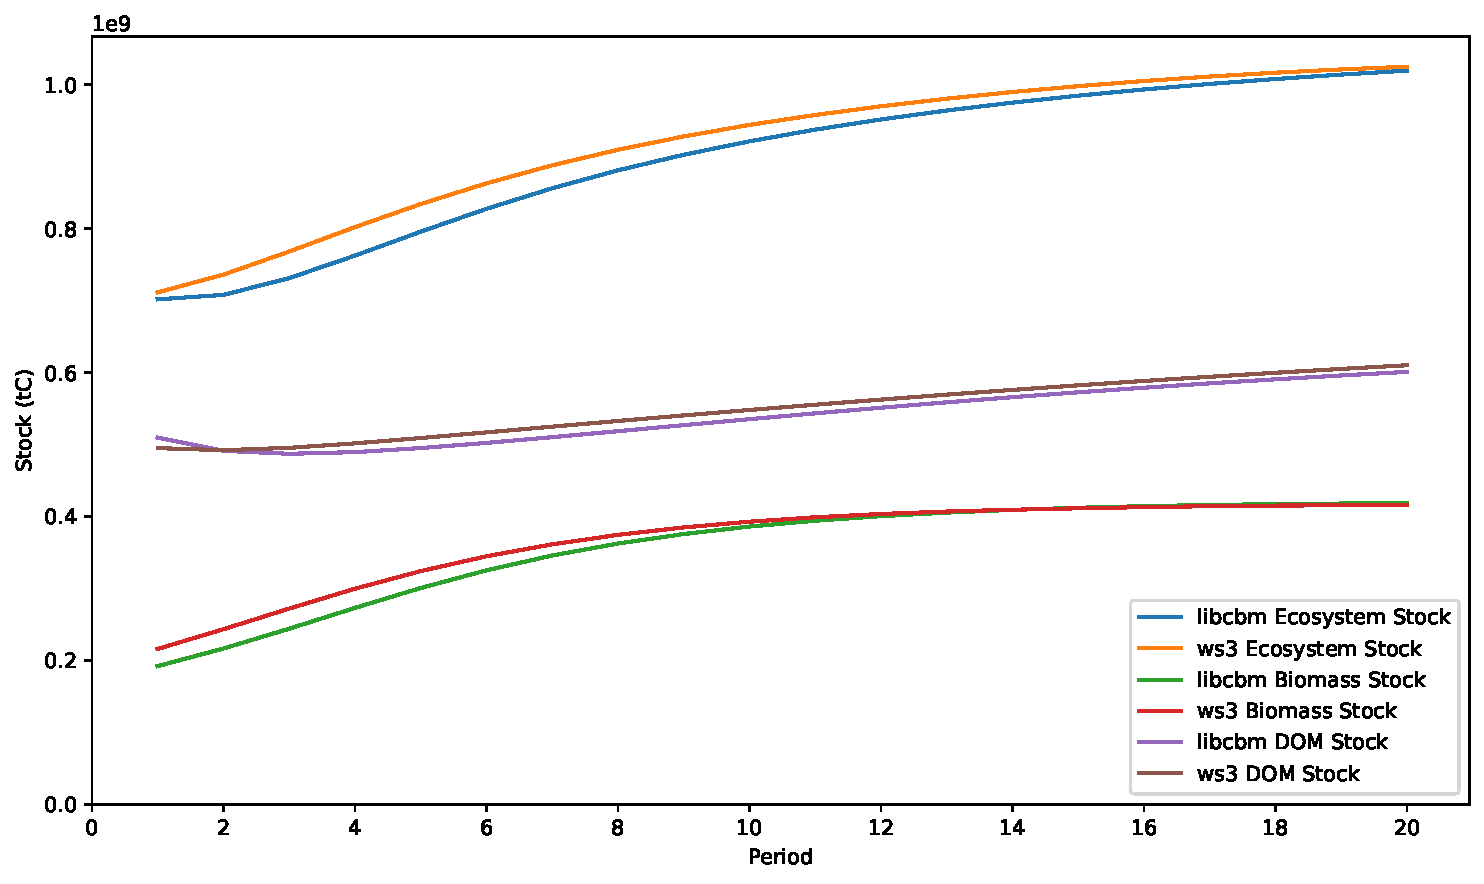
\includegraphics[width=1\linewidth]{no_harvest_stock_total_greg.pdf}
    \caption{The total forest carbon stocks over the 200-year period under no-harvest scenario.}
    \label{fig: nh_stock}
\end{figure}
Figure \ref{fig: nh_emissions} illustrates the results for total carbon emissions from the forest ecosystem under the no-harvest scenario. Initially, the emission starts at a relatively high value of $-9.11 \times 10^{5}$ t$ \mathrm{CO}_2 $, which rapidly decreases to $-4.25 \times 10^{6}$ t$ \mathrm{CO}_2 $ over the first five periods. Subsequently, the sequestration rate slows, and the emissions gradually increase to $-4.03 \times 10^{5}$ t$ \mathrm{CO}_2 $ over the next 15 decades.

\begin{figure}
    \centering
    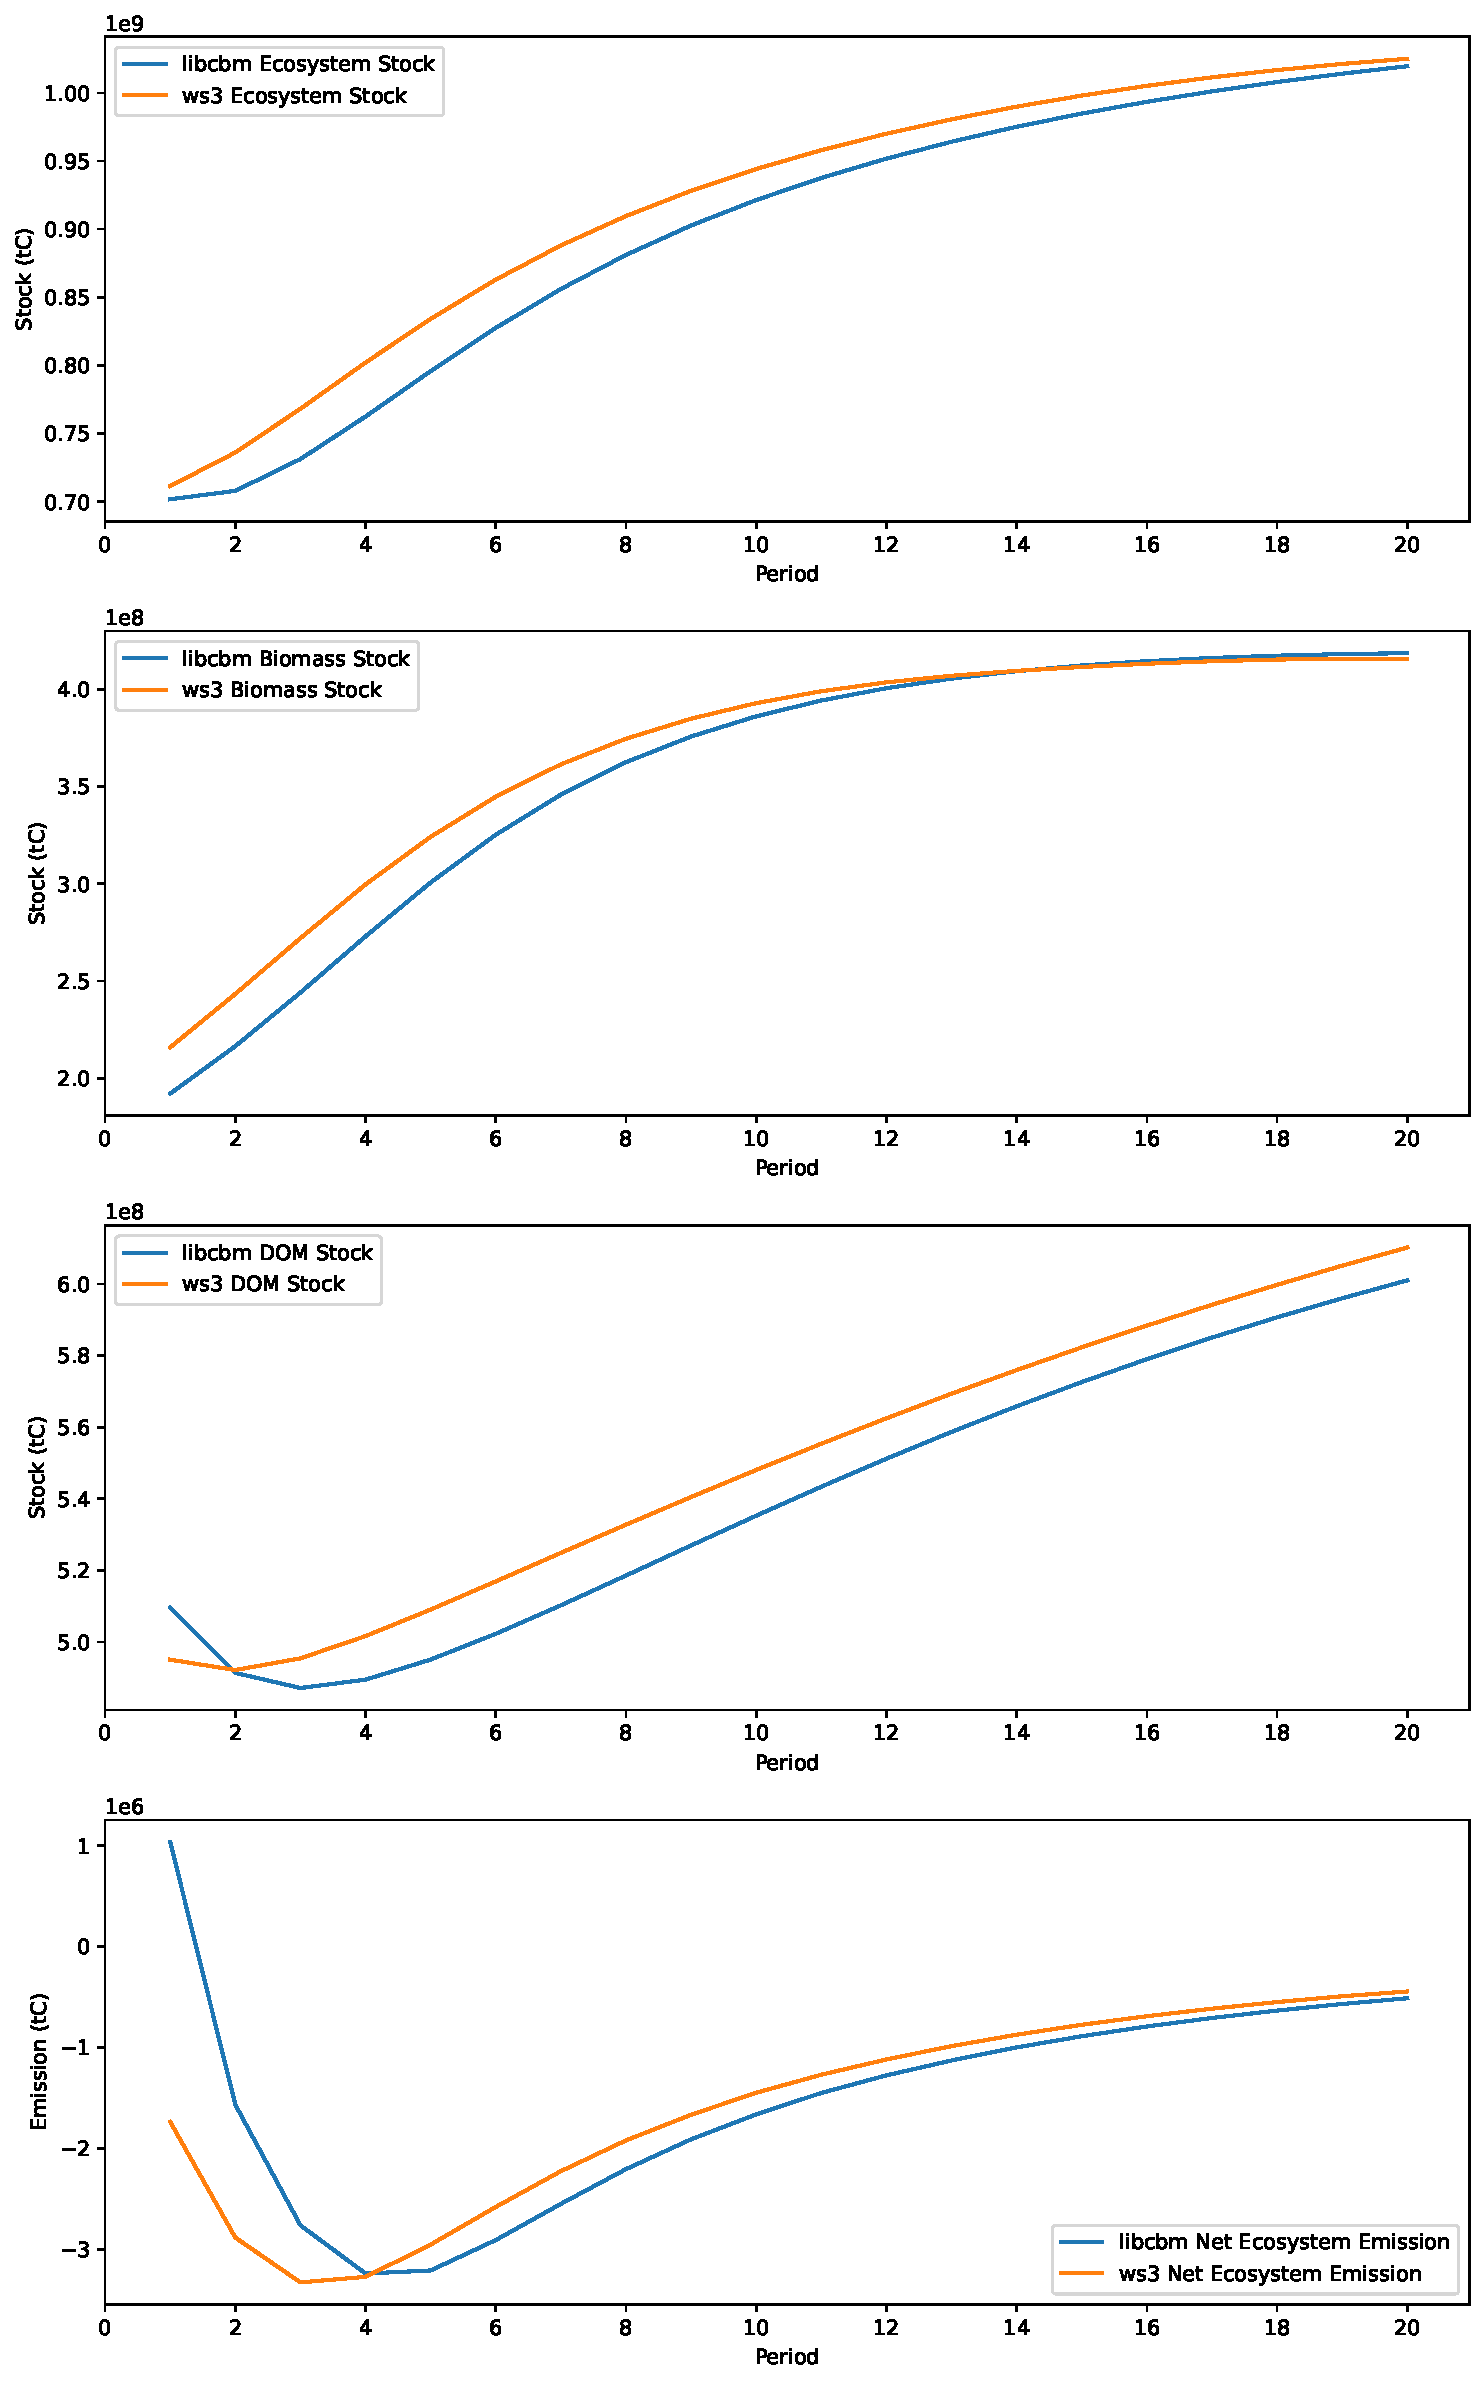
\includegraphics[width=1\linewidth]{emission_nh.pdf}
    \caption{Total forest carbon emissions over the 200-year period under maximize-harvest scenario.}
    \label{fig: nh_emissions}
\end{figure}

Both models show consistent trends for carbon stocks and emissions. In both models, the projected trajectories for biomass carbon are identical, while the average difference of 1.17\% for the \ac{DOM} stock between two models. In total, the proposed model projects lower values of ecosystem stocks during the first 13 periods but higher values in the last 7 periods.

In the max-harvest scenario, the developed model projects lower values of ecosystem stocks than libcbm during the first 13 periods but higher values in the last 7 periods (Figure \ref{fig: st_mh}). Similarly, our model initially projects a lower \ac{DOM} stock, which declines until period 9 before gradually increasing until the end of the planning horizon.  The average percentage differences are $\pm$ 1.04\% for the ecosystem stock, $\pm$ 0.06\% for the biomass stock, and $\pm$ 1.17\% for the \ac{DOM} stock. demonstrating that the integration of the carbon indicator at the landscape level remains robust, even under scenarios of intensive harvest.
\begin{figure}
    \centering
    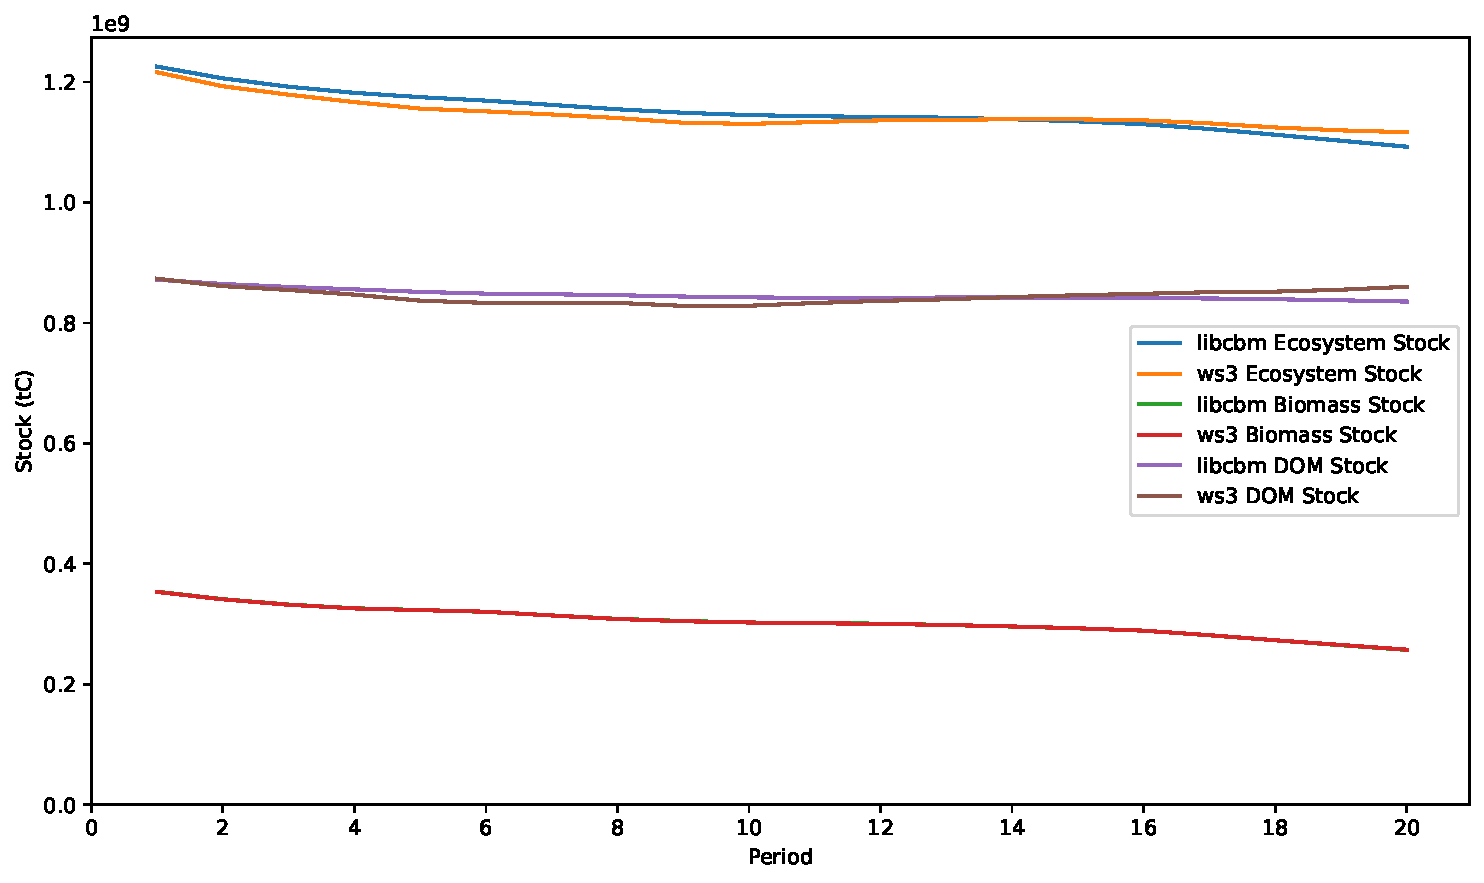
\includegraphics[width=1\linewidth]{maximize_harvest_stock_total.pdf}
    \caption{Total forest carbon stocks over the 200-year period under maximize-harvest scenario.}
    \label{fig: st_mh}
\end{figure}

Despite the close results for the carbon stocks, the developed model consistently underestimate at the beginning and then overestimate net emission in the simulation horizon, with deviations reaching up to 100\% (Figure \ref{fig: em_mh}). 
\begin{figure}
    \centering
    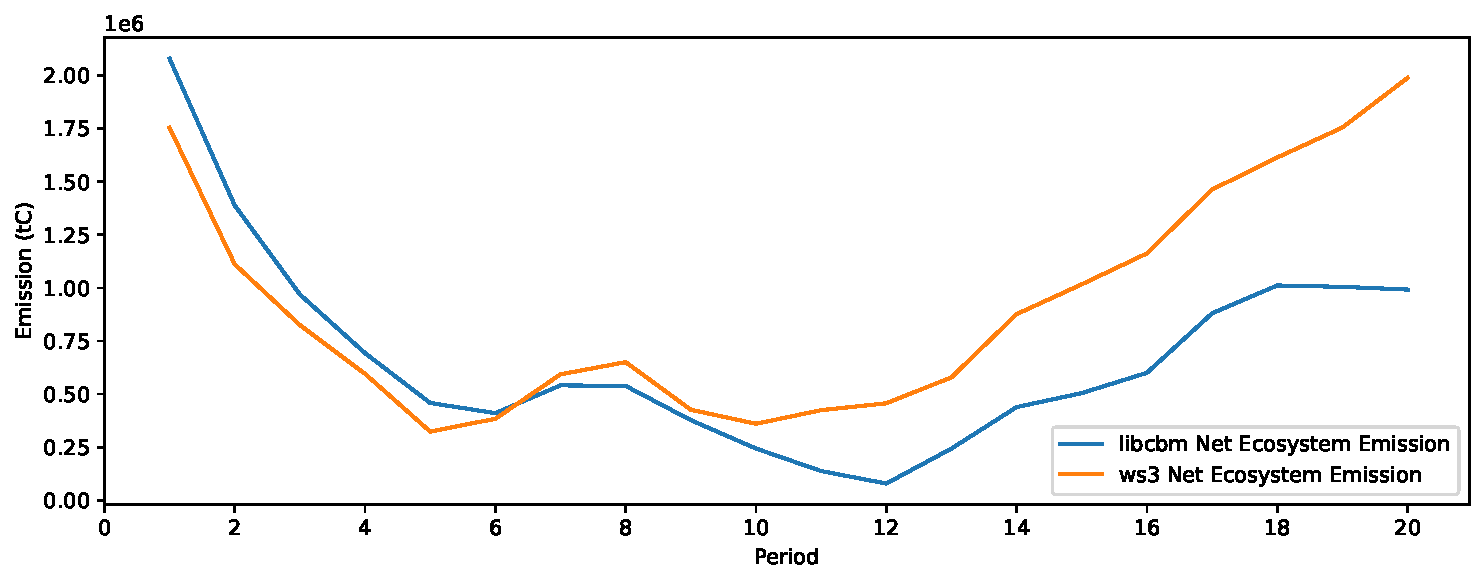
\includegraphics[width=1\linewidth]{emission_mh.pdf}
    \caption{Total forest carbon emissions over the 200-year period under maximize-harvest scenario.}
    \label{fig: em_mh}
\end{figure}

\acp{HWP} and displacement are also crucial in carbon accounting analysis. The outputs from the bi-objective optimization model shows the results of the assessment for a combination of half-lives and displacement factors (Figure \ref{fig: trade_off} ). Figure \ref{fig: trade_off} reveals that there is a trade-off between harvest volume and net negative emissions and when the half-life and displacement factor increase, the trade-off curves shift toward the upper-right portion of the plot and become increasingly horizontal.
\begin{figure}
    \centering
    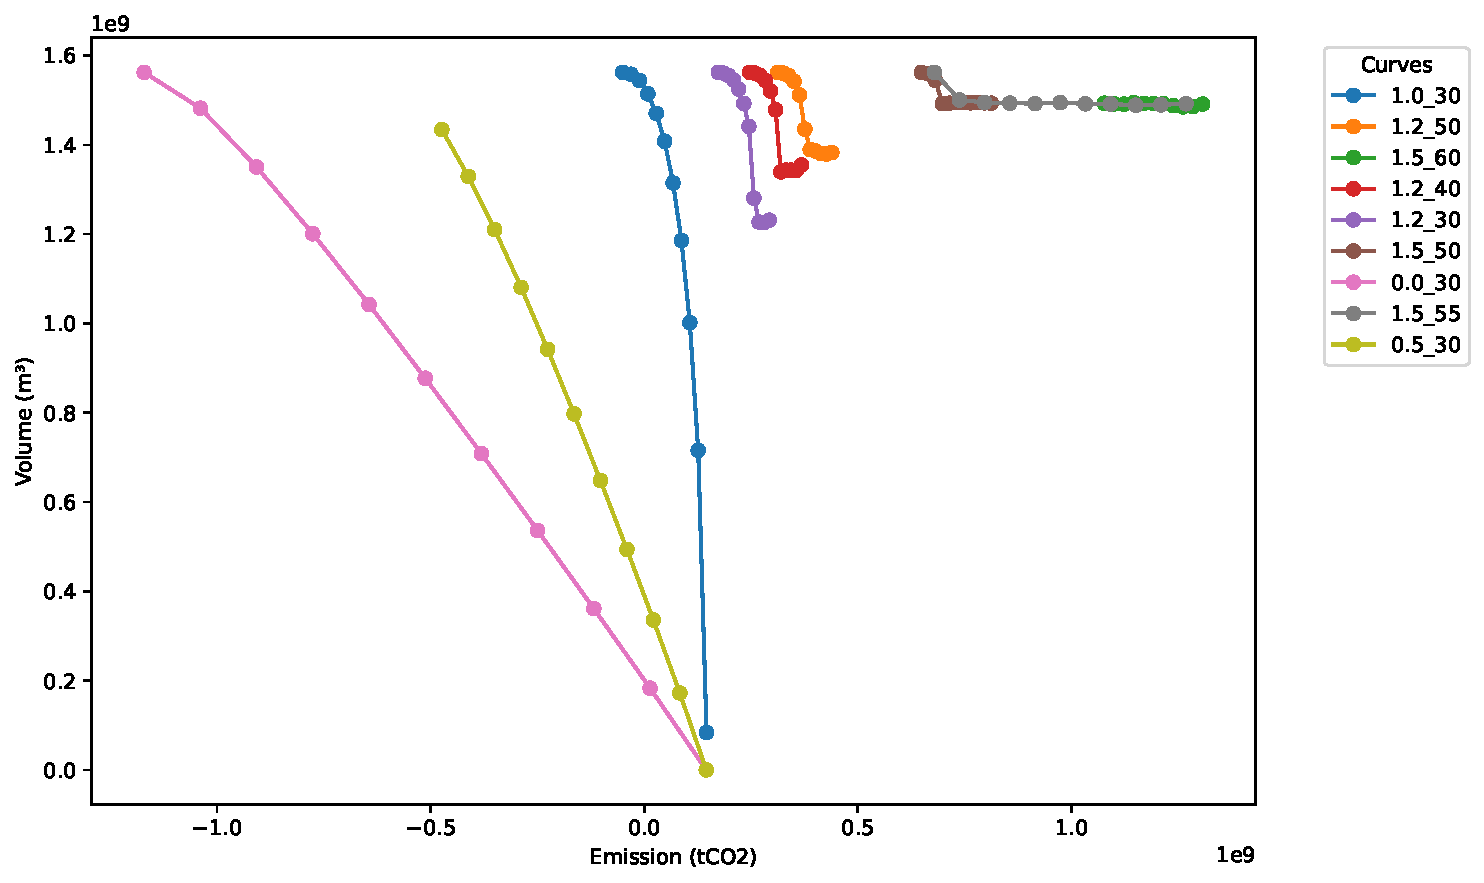
\includegraphics[width=1\linewidth]{tradoff_curves_me.pdf}
    \caption{Trade-off curves between maximizing wood supply and maximizing negative
net carbon emission with varied HWP half-lives and displacement factors (curve name =
displacement factor + half-life).}
    \label{fig: trade_off}
\end{figure}

The results are presented in Figure \ref{fig: 3d_graph}. The results show a clear relationship between these two parameters and the model’s decision to harvest. In the dark blue region, the total harvest volume remains at zero. As either parameter increases, the model begins selecting harvest options, with the total volume rising sharply, forming a cliff pattern on the surface. In this transitional region (which is mostly the result of displacement factors between 0.6 and 1.5 tC / tC and the half-life between 0-200 years), the harvest volume increases rapidly from 0 to greater than $1.2 \times 10^9$ m$^3$, creating an unstable zone with high output sensitivity (top view in Figure \ref{fig: 2d_graphs}).

In Figure \ref{fig: 2d_graphs}, the side view shows the isolated influence of half-life, keeping the displacement factor constant along the y-axis. Here, total harvest volume remains low when the half-life is below 50 years, but increases sharply between 75–125 years, particularly when the displacement factor is high. The total volume reaches over $1.4 \times 10^9$ m$^3$ when the half-life exceeds 150 years with a medium level of displacement factor (around 1.1 tC/tC).

The front view in \ref{fig: 2d_graphs} highlights the effect of the displacement factor, with half-life held constant on the x-axis. When the displacement factor is below 0.6 tC/tC, the harvest volume stays near 0, even with half-lives up to 200 years. In contrast, displacement factors above 1.0 tC/tC result in a substantial increase in harvest volume, especially for moderate-to-high half-lives. Once the displacement factor exceeds 1.5 tC/tC, the model opts for nearly full harvest volume (above $1.4 \times 10^9$ m$^3$) even when the half-life is 0.
\begin{figure}
    \centering
    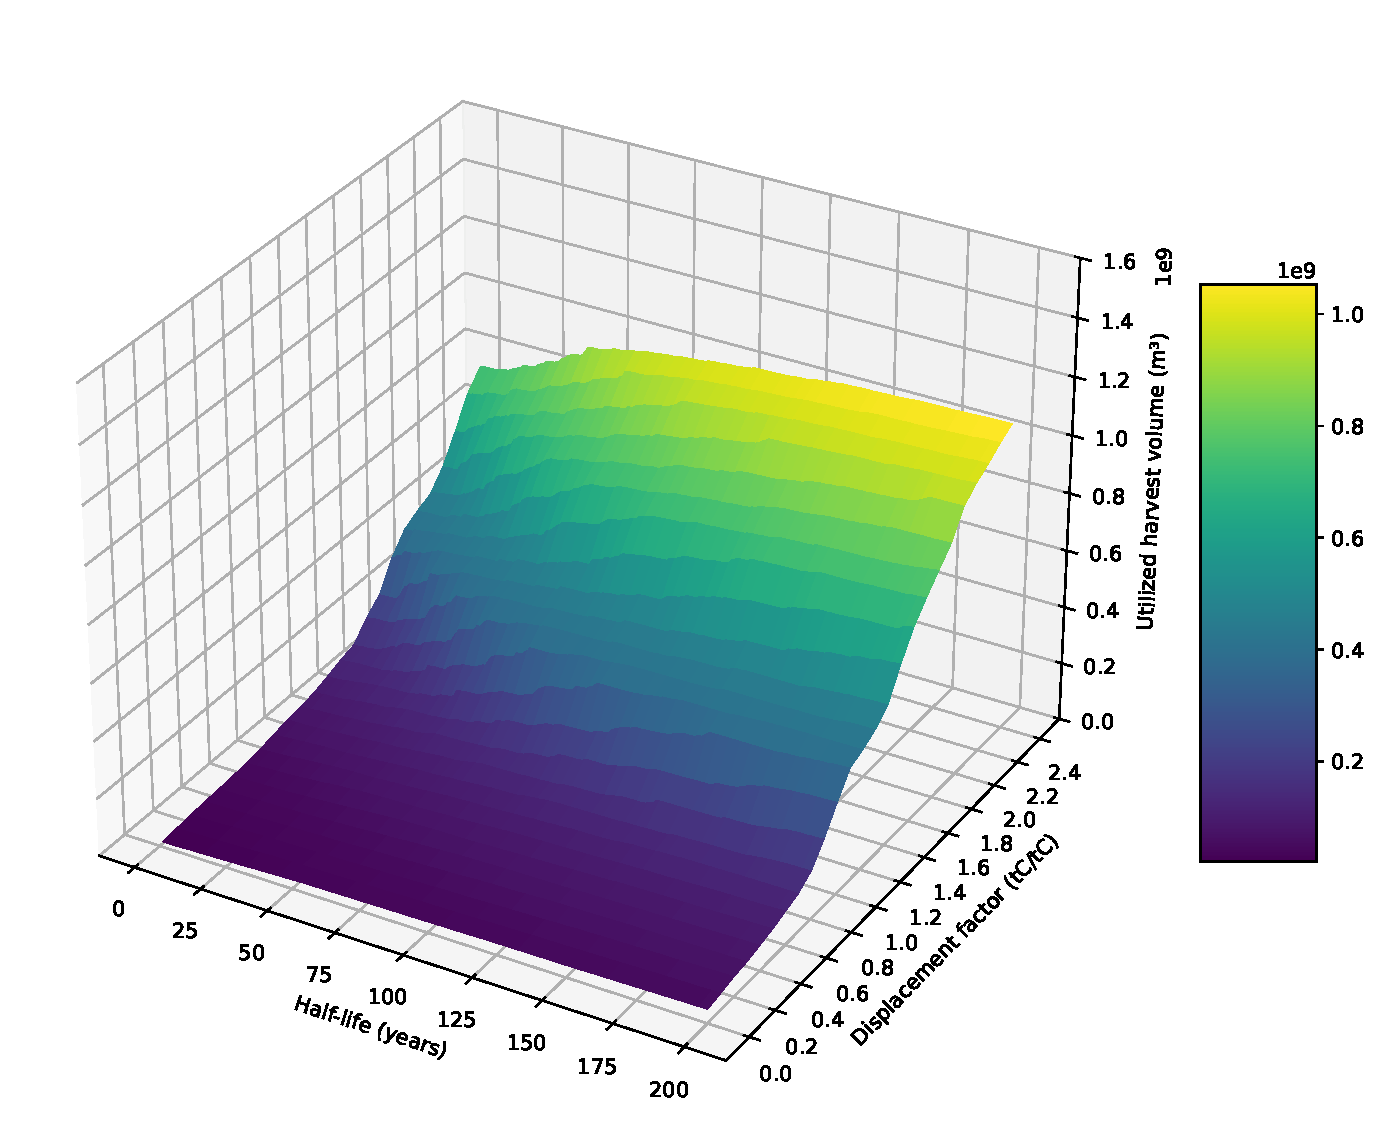
\includegraphics[width=1\linewidth]{3d.pdf}
    \caption{3D mapping of model sensitivity to HWP half-life and displacement factor.}
    \label{fig: 3d_graph}
\end{figure}

\begin{figure}
    \centering
    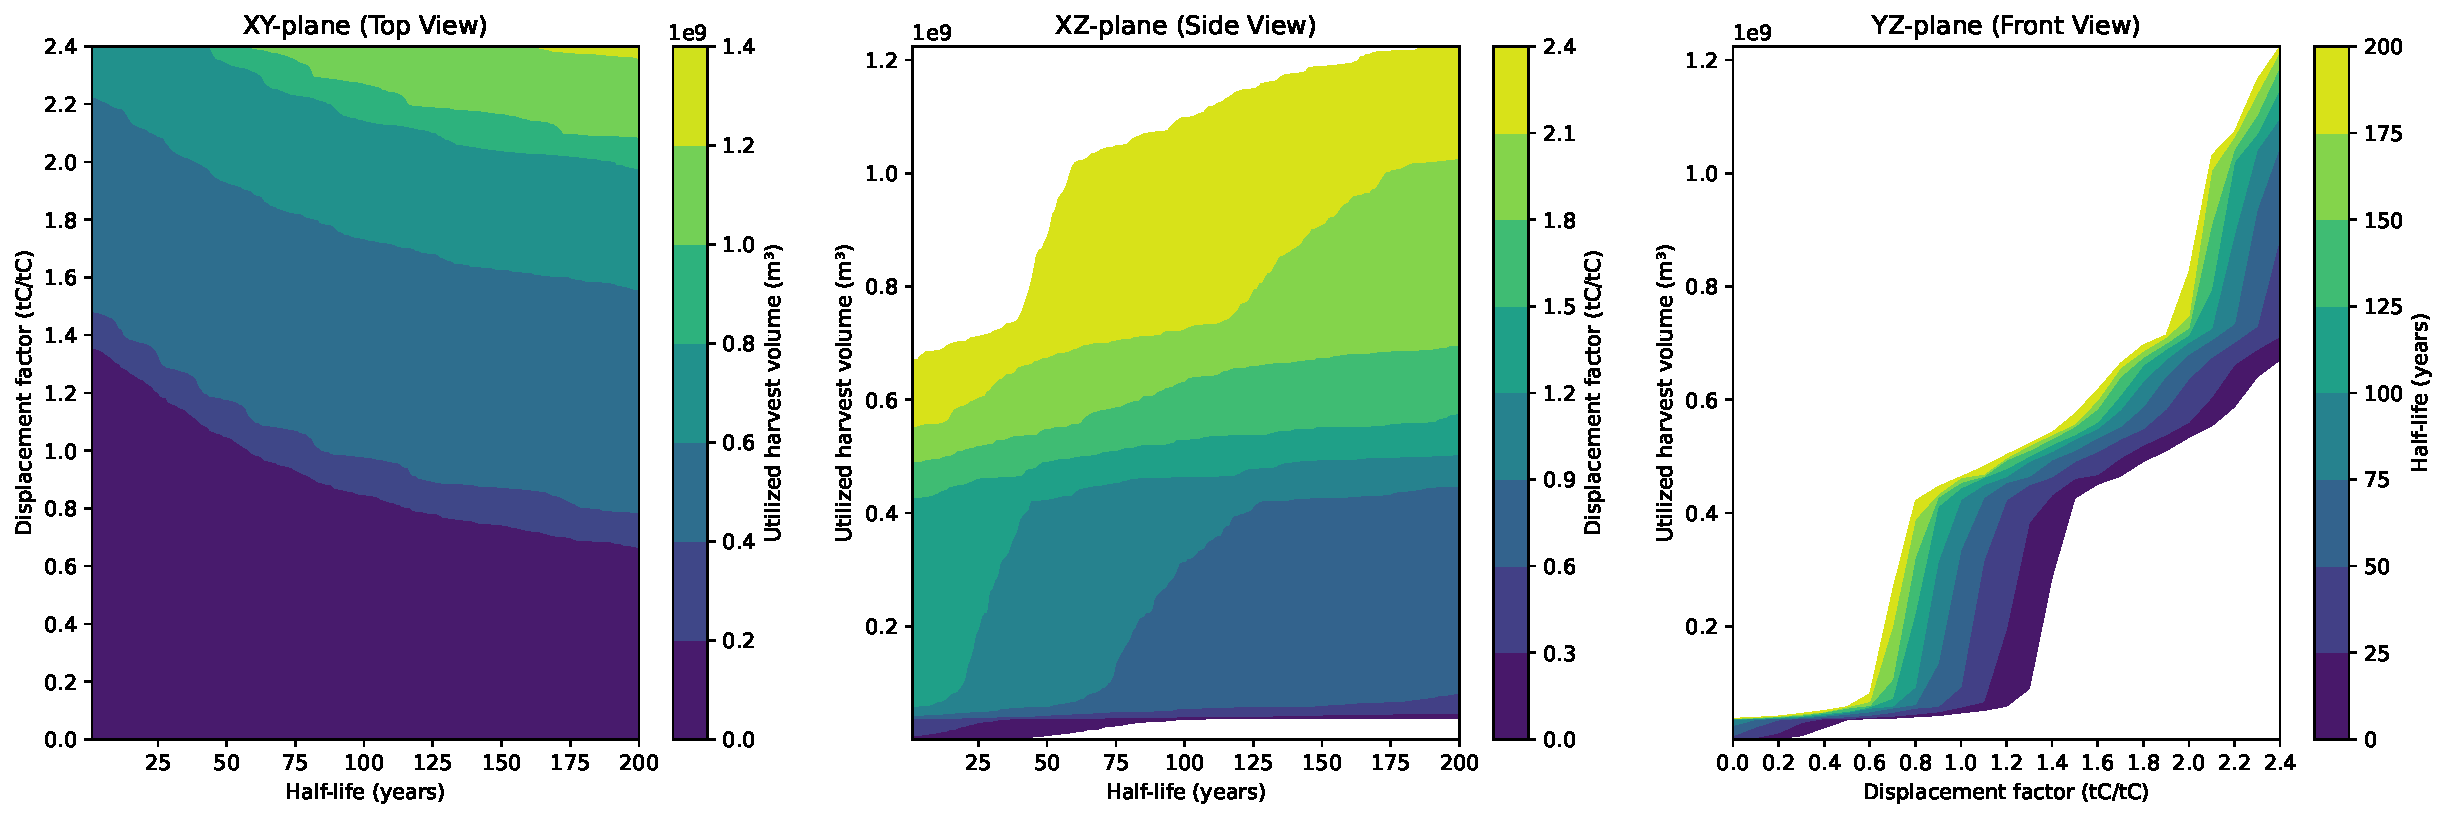
\includegraphics[width=1\linewidth]{xyz.pdf}
    \caption{Orthographic views of 3D mapping of model sensitivity to HWP half-life and displacement factor.}
    \label{fig: 2d_graphs}
\end{figure}


\section{Discussion}
\label{sec:discussion}
\subsection{Model Performance}
When the \ac{SFMM} was set to maximize the harvested timber volume (Figure \ref{fig: area_vol_stock}), the even-flow constraints act as imposed limits on the harvest area ($ha$). This causes limited variation and stability in the harvested area and harvested timber volume over the 200-year planning horizon. 

Although our model and libcbm use similar inputs such as forest inventory, yield curves, and treatment transitions to estimate forest carbon dynamics, they differ fundamentally in the forest carbon modeling mechanism, which can potentially lead to divergent outputs. libcbm includes a built-in carbon accounting framework that explicitly simulates fluxes between carbon pools and tracks carbon stocks using deterministic logic parametrized by either built-in default or user-override flux logic parameters \citep{libcbmpy}. In contrast, our model lacks an internal carbon model and instead relies on carbon stock and flux yield curves generated from libcbm as an approximation.

There are several policy-making insights from the forest management perspective. As observed in the age distributions (Figures \ref{fig: unmanaged age structure}, \ref{fig: managed age structure}), the unmanaged forests are shaped by natural disturbances rather than silvicultural interventions, while managed forests are formed by decades of harvesting, planing, and stand-replacing treatments. These differences between managed and unmanaged forests have direct implications for carbon dynamics. Managed forests may support higher short-term carbon sequestration rates due to rapid biomass accumulation in young stands, but unmanaged forests can contribute substantially to long-term carbon storage through older, high-biomass stands. Furthermore, unmanaged forests offer important structural complexity and ecological functions that support habitat diversity and long-term ecosystem stability \citep{sutherland2016recovery}.

The comparisons between our model and libcbm reveal the reliability and robustness of the developed model. In the no-harvest scenario, the biomass carbon dynamics mirror the changes observed in the growing stock due to the strong correlation between the biomass carbon stock and the wood volume of living trees. The forest ecosystem functioned as a persistent carbon sink, with net emission remaining negative throughout the simulation period, sequestering \ac{CO$_2$} from the atmosphere. The biomass carbon stocks increased rapidly during the initial simulation periods due to forest growth. Meanwhile, the \ac{DOM} stock exhibited a slower but steady increase driven by the dynamics of natural litterfall and decomposition. The carbon yield curve method performed exceptionally well in this scenario, with deviations from libcbm averaging below 0.5\%. This close alignment confirmed that the method succeeded in modeling the carbon dynamics of unmanaged forests at the landscape scale as represented in libcbm. Without harvesting activities, the carbon modeling outputs of the proposed model and libcbm exhibit nearly identical trends, confirming the successful integration of the carbon yield curves into the optimization model (Figure~\ref{fig: nh_stock} and Figure~\ref{fig: nh_emissions})

As shown in Figures \ref{fig: st_mh}, both libcbm and our model have projected relatively similar carbon stocks pools while the most significant divergence occurred in net ecosystem carbon emission (Figure \ref{fig: em_mh}). This likely results from the cumulative effect of how the model resets post-harvest stand age to zero, applying initial values of carbon yield curves, which inflate \ac{DOM} fluxes. Despite these discrepancies, overall emission trends remain aligned across models. As such, it is still feasible to use the model for optimization purposes to optimize forest management decisions considering carbon stocks and emissions.

From a climate change mitigation perspective, two key forest management strategies are widely discussed. One considers forests as carbon reservoirs, where conservation policies aim to preserve and increase forest carbon stocks. The other recommends intensified forest management, producing \acp{HWP} whose use can lead to displacement effects that potentially reduce ecosystem emissions. Within the scientific community, however, there is still no consensus on which approach provides the best climate benefit. A group of studies (e.g. \citep{gustavsson2017climate}, \citep{heinonen2017scenario}) concluded that increasing harvesting level can lead to more climate benefits while other researchers (e.g. \cite{leturcq2020ghg}, \cite{skytt2021climate}, \cite{soimakallio2022closing}) found increased harvesting counterproductive for climate change mitigation. Considering the inherent uncertainty in displacement factor values, this study investigate the forest management under a wide range of possible displacement factors and half-lives. Figure \ref{fig: 3d_graph} offers valuable guidance for policymakers aiming to provide strategies that both contribute to the climate change mitigation and meet business objectives. When half-lives and displacement factors are low, the model identifies a no-harvest approach as optimal, reflecting the limited ability of \acp{HWP} to offset the emissions generated by harvesting. In contrast, when both values are high, maximizing harvest becomes the preferred policy. This reflects the critical role of long-lived \acp{HWP} with strong substitution effects. In practice, forest management approaches that prioritize producing durable wood products capable of replacing more carbon-intensive materials can help bridge the gap between economic and climate goals. 

Figure \ref{fig: 3d_graph} also shows that, among the input parameters, the displacement factor is more sensitive than the half-life. Moreover, there is a narrow, unstable transition region where even small changes in either parameter can lead to a sudden shift in the optimal policy from a no-harvest to a max-harvest scenario. This implies that there is no “one-size-fits-all” solution for forest management, as policies are highly sensitive to underlying uncertainties in the downstream forest supply chain. Such uncertainties can originate from various sources. For instance, changes in trade tariffs or fluctuations in fibre demand can significantly influence \acp{HWP} production, ultimately reshaping forest management strategies.


\section{Conclusion}
\label{sec:conclusion}
\newpage



\section*{CRediT authorship contribution statement}
\label{sec: CRediT}


\section*{Declaration of competing interest}
\label{sec:Declaration of Competing Interest}
The authors declare that they have no known competing financial interests or personal relationships that could have appeared to influence the work reported in this article.

\section*{Acknowledgments}
\label{sec:acknowledgments}
This work was supported by ...


\section*{Data availability statement}
\label{sec: data availability}
The data and code supporting the findings of this study are available in ?. 
\end{linenumbers}
%% If you have bibdatabase file and want bibtex to generate the
%% bibitems, please use
%%
\bibliographystyle{elsarticle-harv} 
\bibliography{reference}

%% else use the following coding to input the bibitems directly in the
%% TeX file.


%% The Appendices part is started with the command \appendix;
%% appendix sections are then done as normal sections
\appendix

\section{Appendix}
\label{sec: appendix}

\end{document}

\endinput
%%
%% End of file `manuscript.tex'.